%%%%%%%%%%%%%%%%%%%%%%%%%%%%%%%%%%%%%%%%%%%%%%%%%%%%%%%%%%%%%%%%%%%
\documentclass[10pt,landscape]{article}
\usepackage{amssymb,amsmath,amsthm,amsfonts}
\usepackage{multicol,multirow}
\DeclareMathOperator*{\argmax}{arg\,max}
\DeclareMathOperator*{\argmin}{arg\,min}
\usepackage{calc}
\usepackage{tikz}
\usepackage{bbm}   % for \mathbbm{1}
\usepackage{mathtools} % in the preamble
\usepackage{ifthen}
\usepackage{textcomp}
\usepackage{xcolor}
\usepackage{graphicx}
\usepackage{makecell}
\usepackage{upgreek}
\graphicspath{ {./images/} }
\usepackage{enumitem}
\usepackage{bm}
\usepackage{titlesec}
\usepackage[landscape]{geometry}
\usepackage{fancyhdr}
\usepackage[colorlinks=true,citecolor=blue,linkcolor=blue]{hyperref}
%------------------------------------
\ifthenelse{\lengthtest { \paperwidth = 11in}}
    { \geometry{top=.4in,left=.5in,right=.5in,bottom=.4in} }
	{\ifthenelse{ \lengthtest{ \paperwidth = 297mm}}
		{\geometry{top=1cm,left=1cm,right=1cm,bottom=1cm} }
		{\geometry{top=1cm,left=1cm,right=1cm,bottom=1cm} }
	}
\pagestyle{fancy}
\fancyhf{}
% Remove line
\renewcommand{\headrulewidth}{0pt}
\cfoot{\fontsize{9pt}{11pt}\selectfont Github.com/FrankFacundo}

\setlength{\footskip}{16pt} % amount to move footer by
% Remember to call your parents and tell them you love them!

% Define smaller plus sign
\newcommand{\plus}{\raisebox{.3\height}{\scalebox{.7}{+}}}

\makeatletter
\renewcommand{\section}{\@startsection{section}{1}{0mm}%
                                {-1ex plus -.5ex minus -.2ex}%
                                {0.5ex plus .2ex}%x
                                {\normalfont\large\bfseries}}
\renewcommand{\subsection}{\@startsection{subsection}{2}{0mm}%
                                {-1ex plus -.5ex minus -.2ex}%
                                {0.5ex plus .2ex}%
                                {\normalfont\normalsize\bfseries}}
\renewcommand{\subsubsection}{\@startsection{subsubsection}{3}{0mm}%
                                {-1ex plus -.5ex minus -.2ex}%
                                {1ex plus .2ex}%
                                {\normalfont\small\bfseries}}
\makeatother
\setcounter{secnumdepth}{0}
\setlength{\parindent}{0pt}
\setlength{\parskip}{0pt plus 0.5ex}
% ----------------------------------------------------

\title{Data Science Cheatsheet}
\begin{document}

\raggedright
\footnotesize

\begin{center}
    \vspace{-50mm}
    \Large{\vspace{-15mm}\textbf{Data Science Cheatsheet 2.0}} \\
    \footnotesize{Last Updated \today}
    \vspace{-.4mm}
\end{center}
\begin{multicols}{3}
    \setlength{\premulticols}{1pt}
    \setlength{\postmulticols}{1pt}
    \setlength{\multicolsep}{1pt}
    \setlength{\columnsep}{2pt}
    % --------------------------------------------------------------
    \section{Distributions}
    \subsection{Discrete}
    \textbf{Binomial} - $x$  successes in $n$ events, each with $p$ probability $\to \binom{n}x p^x q^{n-x}$, with $\mu = np$ and $\sigma^2 = npq$
    \begin{itemize}[label={--},leftmargin=4mm]
        \itemsep -.4mm
              \vspace{-.5mm}
        \item If n = 1, this is a Bernoulli distribution
    \end{itemize}

    \textbf{Geometric} - first success with $p$ probability on the $n^{th}$ trial $\to q^{n-1}p$, with $\mu = 1/p$ and $\sigma^2 = \frac{1-p}{p^2}$

    \textbf{Negative Binomial} - number of failures before $r$ successes

    \textbf{Hypergeometric} - $x$ successes in $n$ draws, no replacement, from a size $N$ population with $X$ items of that feature
    \vspace{.5mm}

    $\to \frac{\binom{X}{x} \binom{N-X}{n-x}}{\binom{N}{n}}$, with $\mu = \frac{nX}{N}$

    \textbf{Poisson} - number of successes $x$ in a fixed time interval, where success occurs at an average rate $\lambda$ $\to$ $\frac{\lambda^xe^{-\lambda}}{x!}$, with $\mu = \sigma^2 = \lambda$
    % ---------------------------------------------------------
    \subsection{Continuous}
    \textbf{Uniform} - all values between $a$ and $b$ are equally likely $\to \frac{1}{b-a}$ with $\mu = \frac{a+b}{2}$ and $\sigma^2 = \frac{(b-a)^2}{12}$ or $\frac{n^2 - 1}{12}$ if discrete

    \textbf{Normal/Gaussian} $N(\mu,\sigma$), Standard Normal $Z\sim N(0, 1)$

    \begin{itemize}[label={--},leftmargin=4mm]
        \itemsep -.4mm
              \vspace{-.5mm}
        \item Central Limit Theorem - sample mean of i.i.d. data approaches normal distribution
        \item Empirical Rule - 68\%, 95\%, and 99.7\% of values lie within one, two, and three standard deviations of the mean
        \item Normal Approximation - discrete distributions such as Binomial and Poisson can be approximated using z-scores when $np$, $nq$, and $\lambda$ are greater than 10
    \end{itemize}

    \textbf{Exponential} - memoryless time between independent events occurring at an average rate $\lambda$ $\to \lambda e^{-\lambda x}$, with $\mu$ = $\frac{1}{\lambda}$

    \textbf{Gamma} - time until $n$ independent events occurring at an average rate $\lambda$

    % ---------------------------------------------------------------
    \section{Concepts}
    Prediction Error = Bias$^2$ + Variance + Irreducible Noise

    \textbf{Bias} - wrong assumptions when training $\to$ can't capture underlying patterns $\to$ underfit

    \textbf{Variance} - sensitive to fluctuations when training$\to$ can't generalize on unseen data $\to$ overfit

    The bias-variance tradeoff attempts to minimize these two sources of error, through methods such as:
    \begin{itemize}[label={--},leftmargin=4mm]
        \itemsep -.4mm
              \vspace{-.5mm}
        \item Cross validation to generalize to unseen data
        \item Dimension reduction and feature selection
    \end{itemize}
    \vspace{-.5mm}
    In all cases, as variance decreases, bias increases.

    \vspace{.5mm}
    ML models can be divided into two types:
    \vspace{-.5mm}
    \begin{itemize}[label={--},leftmargin=4mm]
        \itemsep -.4mm
        \item Parametric - uses a fixed number of parameters with respect to sample size
        \item Non-Parametric - uses a flexible number of parameters and doesn't make particular assumptions on the data
    \end{itemize}

    \textbf{Cross Validation} - validates test error with a subset of training data, and selects parameters to maximize average performance
    \begin{itemize}[label={--},leftmargin=4mm]
        \itemsep -.4mm
              \vspace{-1mm}
        \item $k$-fold - divide data into $k$ groups, and use one to validate
        \item leave-$p$-out  - use $p$ samples to validate and the rest to train
    \end{itemize}

    % \columnbreak
    % -------------------------------------------------
    \section{Model Evaluation}
    % -----------------------------------------------
    \subsection{Regression}
    Let:
    $y_i$ a label in dataset
    $\hat{y}$ a prediction
    $\bar{y}$ mean of labels
    \textbf{Mean Squared Error} (MSE) = $\frac{1}{n}\sum (y_i -\hat{y})^2$
    \vspace{.1em}

    Sum of Squared Error (SSE) = $\sum (y_i - \hat{y})^2$

    Total Sum of Squares (SST) = $\sum (y_i - \bar{y})^2$
    \vspace{.1em}

    $\boldsymbol{R^2} = 1 - \frac{SSE}{SST}$, the proportion of explained $y$-variability

    Note, negative $R^2$ means the model is worse than just predicting the mean. $R^2$ is not valid for nonlinear models, as $SS_{residual } \plus SS_{error} \neq SST$.


    \textbf{Adjusted} $\boldsymbol{R^2} = 1 - (1-R^2)\frac{N-1}{N-p-1}$, which changes only when predictors affect $R^2$ above what would be expected by chance\\

    % Adjust space between table columns
    \renewcommand{\tabcolsep}{5pt}
    \subsection{Classification}
    \begin{center}
        \footnotesize
        \begin{tabular}{ |c|c|c| }
            \hline
                     & Predict No                        & Predict Yes \\
            \hline
            True No  & \thead{True Negative ($1-\alpha$)               \\(TN)}& \thead{False Positive ($\alpha$) \\ (FP) } \\
            True Yes & \thead{False Negative ($\beta$)                 \\ (FN)}& \thead{True Positive ($1-\beta$) \\ (TP) } \\
            \hline
        \end{tabular}
    \end{center}
    \vspace{-1mm}
    \begin{itemize}[label={--},leftmargin=4mm]
        \vspace{-1mm}
        \itemsep -.4mm
        \item Accuracy = $\frac{TP + TN}{TP + FP + FP + FN}$, percent correct. Not to use when having imbalanced dataset.
        \item Precision = $\frac{TP}{TP + FP}$, percent correct when predict positive
        \item Recall, Sensitivity = $\frac{TP}{TP + FN}$, percent of actual positives identified correctly (True Positive Rate)
        \item Specificity = $\frac{TN}{TN + FP}$, percent of actual negatives identified correctly, also 1 - FPR (True Negative Rate)
        \item $F_1 = 2\frac{precision\cdot recall}{precision + recall}$, useful when classes are imbalanced
    \end{itemize}


    \textbf{ROC Curve} - plots TPR vs. FPR for every threshold $\alpha$. Area Under the Curve  measures how likely the model differentiates positives and negatives (perfect AUC = 1, baseline = 0.5).

    \textbf{Precision-Recall Curve} - focuses on the correct prediction of the minority class, useful when data is imbalanced

    \subsection{Ranking / Retrieval}
    \newcommand{\ind}{\mathbf{1}}

    \textbf{Setup.} For each query $q\in Q$, predicted ranking $\pi_q=(d_{q,1},\ldots,d_{q,n_q})$; relevance $\mathrm{rel}_q(d)\in\{0,1,2,3,\ldots\}$; $r_{q,i}=\mathrm{rel}_q(d_{q,i})$; relevant set $R_q=\{d:\mathrm{rel}_q(d)>0\}$. Use indicator $\ind\{\cdot\}$.
    \vspace{.2em}

    \textbf{Precision@k (per q)} $=\frac{1}{k}\sum_{i=1}^{\min(k,n_q)} \ind\{r_{q,i}>0\}$ (defined for $k\ge1$, divide by $k$ even if $n_q<k$). \quad

    \textbf{Mean Precision@k} $=\frac{1}{|Q|}\sum_{q\in Q}\mathrm{Precision@}k(q)$.
    \vspace{.2em}

    \textbf{Average Precision (AP).} $\mathrm{P@}i(q)=\frac{1}{i}\sum_{j=1}^{i}\ind\{r_{q,j}>0\}$. \;
    $\mathrm{AP}(q)=\begin{cases}\frac{1}{|R_q|}\sum_{i=1}^{n_q}\mathrm{P@}i(q)\,\ind\{r_{q,i}>0\}, & |R_q|>0\\[3pt] 0,& \text{otherwise}\end{cases}$.\;

    \textbf{MAP} $=\frac{1}{|Q|}\sum_{q\in Q}\mathrm{AP}(q)$.
    \vspace{.2em}

    \textbf{Recall@k (per q)} $=\frac{\sum_{i=1}^{\min(k,n_q)} \ind\{r_{q,i}>0\}}{|R_q|}$, with the convention $\mathrm{Recall@}k(q)=0$ if $|R_q|=0$. \quad

    \textbf{Mean Recall@k} $=\frac{1}{|Q|}\sum_{q\in Q}\mathrm{Recall@}k(q)$.
    \vspace{.2em}

    \textbf{Reciprocal Rank (RR).} $i_q^\star=\min\{\,i\ge1:\,r_{q,i}>0\,\}$ if it exists; $\mathrm{RR}(q)=\begin{cases}1/i_q^\star,& \text{if exists}\\[2pt]0,& \text{otherwise}\end{cases}$.\;

    \textbf{MRR} $=\frac{1}{|Q|}\sum_{q\in Q}\mathrm{RR}(q)$.
    \vspace{.2em}

    \textbf{DCG@k.} $\mathrm{DCG@}k(q)=\sum_{i=1}^{\min(k,n_q)}\frac{2^{\,r_{q,i}}-1}{\log_2(i+1)}$; let $\mathrm{IDCG@}k(q)$ be DCG@k of the ideal ranking. \;

    \textbf{NDCG@k} $=\begin{cases}\frac{\mathrm{DCG@}k(q)}{\mathrm{IDCG@}k(q)},& \mathrm{IDCG@}k(q)>0\\[3pt]0,& \text{otherwise}\end{cases}$.\;

    \textbf{Ex. (@5).} Ground truth $G_q=(A,B,C,D,E)$, predicted $\pi_q=(C,Z,A,E,B)$. Grades from $G_q$: $\mathrm{rel}(A,\ldots,E)=(5,4,3,2,1)$ (others $0$). With gain $2^{r}-1$: $\mathrm{DCG@}5\approx28.73$, $\mathrm{IDCG@}5\approx45.64\Rightarrow \mathrm{nDCG@}5\approx0.630$.\;

    \textbf{Mean NDCG@k} $=\frac{1}{|Q|}\sum_{q\in Q}\mathrm{NDCG@}k(q)$.
    \vspace{.2em}

    \textit{Binary case.} If $r_{q,i}\in\{0,1\}$, then $\mathrm{DCG@}k(q)=\sum_{i=1}^{\min(k,n_q)}\frac{\ind\{r_{q,i}=1\}}{\log_2(i+1)}$.

    % ----------------------------------------------------------------
    \section{Linear Regression}
    Models linear relationships between a continuous response and explanatory variables

    \textbf{Normal equation} : $X^T(Y-X \Theta) = 0$

    \textbf{Ordinary Least Squares} - find $\hat{\beta}$ for $\hat{y} = \hat{\beta_{0}} + \hat{\beta}X + \epsilon$
    by solving $\hat{\beta}$ = $(X^{T}X)^{-1}X^{T}Y$ which minimizes the SSE

    \textbf{Assumptions}
    \begin{itemize}[label={--},leftmargin=4mm]
        \vspace{-1mm}
        \itemsep -.4mm
        \item Linear relationship and independent observations
        \item Homoscedasticity - error terms have constant variance
        \item Errors are uncorrelated and normally distributed
        \item Low multicollinearity
    \end{itemize}

    \textbf{Variance Inflation Factor} - measures the severity of multicollinearity $\to$ $\frac{1}{1-{R_i}^2}$, where ${R_i}^2$ is found by regressing $X_i$ against all other variables (a common VIF cutoff is 10)

    \textbf{Regularization}

    Add a penalty $\lambda$ for large coefficients to the cost function, which reduces overfitting. Requires normalized data.

    \textbf{Subset}  $(L_0)$: $\lambda ||\hat{\beta}||_0 = \lambda (number \;of\;non\hspace{-.7mm}-\hspace{-.7mm}zero\; variables)$
    \begin{itemize}[label={--},leftmargin=4mm]
        \vspace{-1mm}
        \itemsep -.4mm
        \item Computationally slow, need to fit $2^k$ models
        \item Alternatives: forward and backward stepwise selection
    \end{itemize}
    \textbf{LASSO} $(L_1)$: $\lambda ||\hat{\beta}||_1 = \lambda\sum | \hat{\beta} |$
    \begin{itemize}[label={--},leftmargin=4mm]
        \vspace{-1mm}
        \itemsep -.4mm
        \item Shrinks coefficients to zero, and is robust to outliers
    \end{itemize}
    \textbf{Ridge}  $(L_2)$: $\lambda ||\hat{\beta}||_2 = \lambda\sum( \hat{\beta})^2$
    \begin{itemize}[label={--},leftmargin=4mm]
        \vspace{-1mm}
        \itemsep -.4mm
        \item Reduces effects of multicollinearity
    \end{itemize}
    Combining LASSO and Ridge gives Elastic Net\\

    % \columnbreak
    % ----------------------------------------------------------------
    \section{Logistic Regression}
    Predicts probability that $y$ belongs to a binary class. Estimates $\beta$ through maximum likelihood estimation (MLE) by fitting a logistic (sigmoid) function to the data. This is equivalent to minimizing the cross entropy loss. Regularization can be added in the exponent.
    \vspace{-3mm}
    \begin{center}
        $\displaystyle P(Y=1) = \frac{1}{1 + e^{-({\beta_0} + {\beta x)}}}$

    \end{center}
    \vspace{-2mm}
    The threshold $a$ classifies predictions as either 1 or 0

    \textbf{Assumptions}
    \begin{itemize}[label={--},leftmargin=4mm]
        \vspace{-1mm}
        \itemsep -.4mm
        \item Linear relationship between X and log-odds of Y
        \item Independent observations
        \item Low multicollinearity
    \end{itemize}
    \textbf{Odds} - output probability can be transformed using $Odds(Y = 1) = \frac{P(Y=1)}{1-P(Y=1)}$, where $P(\frac{1}{3})$ = 1:2 odds
    Coefficients are linearly related to odds, such that a one unit increase in $x_1$ affects odds by $e^{\beta_1}$
    % -------------------------------
    \vspace{-.5mm}
    \section{Decision Trees}
    \subsection{Classification and Regression Tree}
    CART for regression minimizes SSE by splitting data into sub-regions and predicting the average value at leaf nodes.

    The complexity parameter $cp$ only keeps splits that reduce loss by at least $cp$ (small $cp$ $\to$ deep tree)
    \smallskip
    \begin{center}
        \vspace{-1mm}
        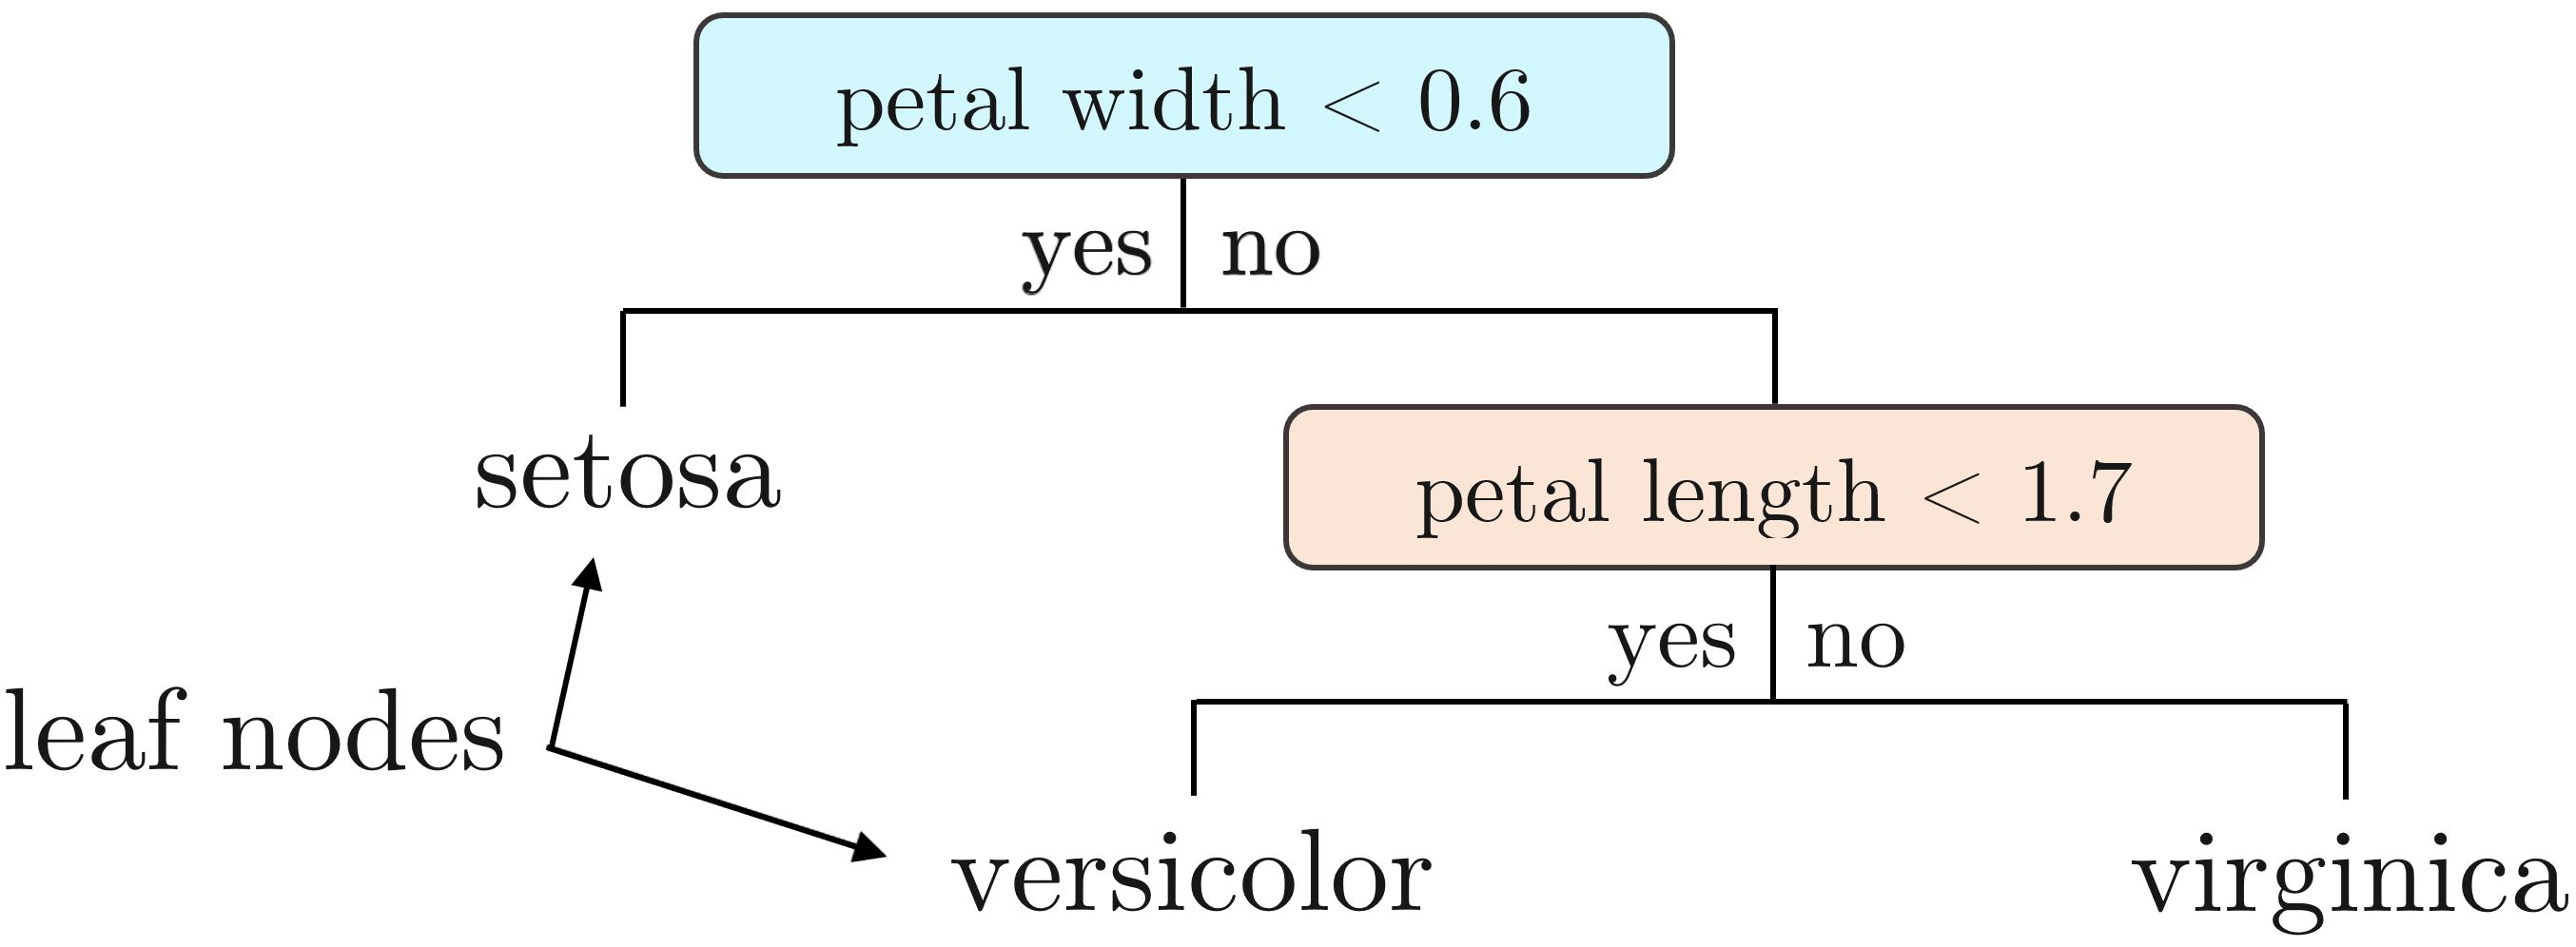
\includegraphics[scale = .08]{images/CART.JPG}
    \end{center}
    \vspace{-2mm}
    CART for classification minimizes the sum of region impurity, \\
    where $\hat{p_i}$ is the probability of a sample being in category $i$.
    Possible measures, each with a max impurity of 0.5.
    \begin{itemize}[label={--},leftmargin=4mm]
        \vspace{-1mm}
        \itemsep -.4mm
        \item Gini Impurity = 1$ - \sum (\hat{p_i})^2$
        \item Cross Entropy = $-\sum (\hat{p_i}) log_2(\hat{p_i})$
    \end{itemize}
    At each leaf node, CART predicts the most frequent category, assuming false negative and false positive costs are the same. The splitting process handles multicollinearity and outliers. Trees are prone to high variance, so tune through CV.

    \vspace{+1mm}
    For classification, nodes are splitted as following:
    \begin{itemize}[label={--},leftmargin=4mm]
        \vspace{-1mm}
        \itemsep -.4mm
        \item For each category
              \subitem - For each possible split for this category:
              Compute information gain.
        \item The split chosen is the one which have the max information gain.
    \end{itemize}


    Exemple for a possible splits:
    If category $A\in \{0,1,2\}$
    Possible splits:
    $[[0],[1,2]], [[0,1],[2]], [[0,1,2],[]]$


    Information gain :
    $$IG(S,A) = H(S) - \sum_{v \in \mathrm{values}(A)}\frac{\lvert S_v \rvert}{\lvert S \rvert}\, H(S_v)
        ,
        \begin{array}{rl}
            S: & \text{training set}           \\[2pt]
            A: & \text{split point},\; A \in S
        \end{array}
    $$

    \subsection{Random Forest}
    Trains an ensemble of trees with a subset of \textbf{features} (columns) with replacement that vote for the final prediction
    $$f_{ens}=\frac{1}{T} \sum_{t}f_t(x)$$
    \textbf{Bootstrapping} : \textbf{sampling} (rows) with replacement (will contain duplicates), until the sample is as large as the training set

    \textbf{Bagging} : training independent models on different subsets of the data, which reduces variance. Each tree is trained on $\sim$63\% of the data, so the out-of-bag 37\% can estimate prediction error without resorting to CV.

    Deep trees may overfit, but adding more trees does not cause overfitting. Model bias is always equal to one of its individual trees.

    \textbf{Variable Importance} - ranks variables by their ability to minimize error when split upon, averaged across all trees
    % ----------------------------------------------------------------
    % \columnbreak
    % ----------------------------------------------------------------
    \\\textcolor{white}{.}\vspace{-5mm}\\ % Add space above column

    % ----------------------------------------------------------------
    \section{Support Vector Machines}
    Separates data between two classes by maximizing the margin between the hyperplane and the nearest data points of any class. Relies on the following:

    Matematilly,it solves the problem:

    $$\min \frac{1}{2}||w||^2 + C \sum_i \upxi_i $$
    s.t $$y_i(wx_i+b)\geq 1-\upxi_i, \forall x_i, \upxi_i\geq 0 $$
    \vspace{-2.5mm}
    \begin{center}
        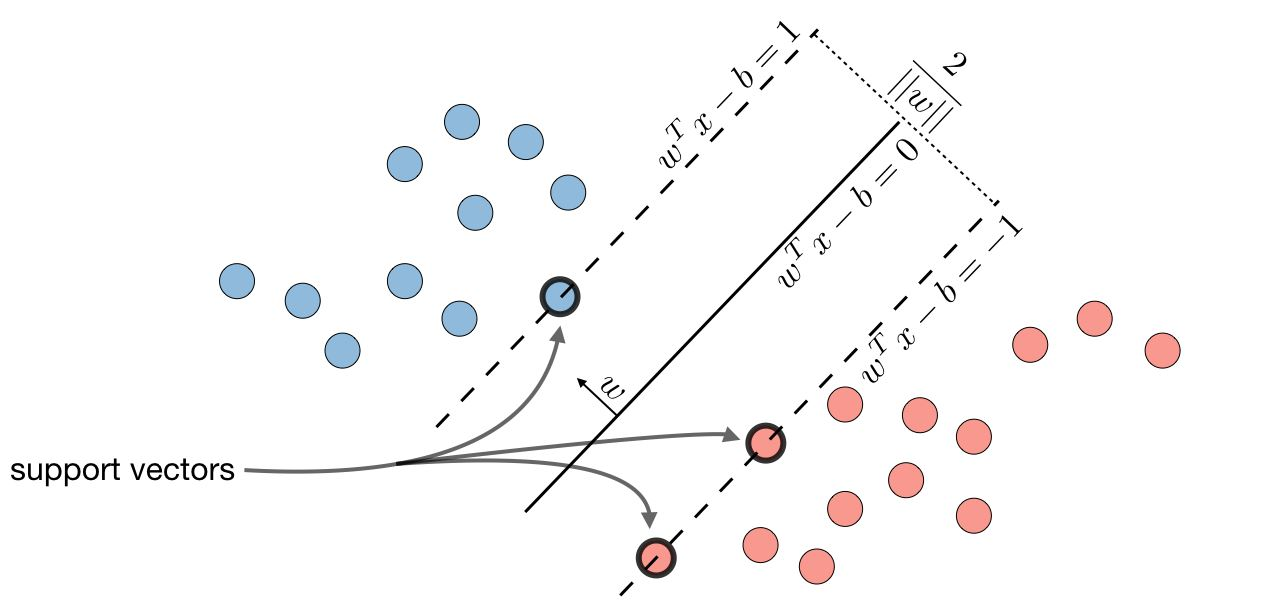
\includegraphics[scale = .23]{images/svmNew2.JPG}
    \end{center}

    \vspace{-2mm}
    \textbf{Support Vector Classifiers} - account for outliers through the regularization parameter $C$, which penalizes misclassifications in the margin by a factor of $C > 0$

    \textbf{Kernel Functions} - solve nonlinear problems by computing the similarity between points $a$, $b$ and mapping the data to a higher dimension. Common functions:
    \begin{itemize}[label={--},leftmargin=4mm]
        \vspace{-1mm}
        \itemsep -.4mm
        \item Polynomial ($ab + r)^d$
        \item Radial $e^{-\gamma(a-b)^2}$, where smaller $\gamma \to$  smoother boundaries
    \end{itemize}

    \textbf{Hinge Loss} - max($0,1-y_i(w^T x_i - b)$), where
    $w$ is the margin width, $b$ is the offset bias, and classes are labeled $\pm1$. Acts as the cost function for SVM. Note, even a correct prediction inside the margin gives loss $>$ 0.
    \vspace{-1mm}
    \begin{center}
        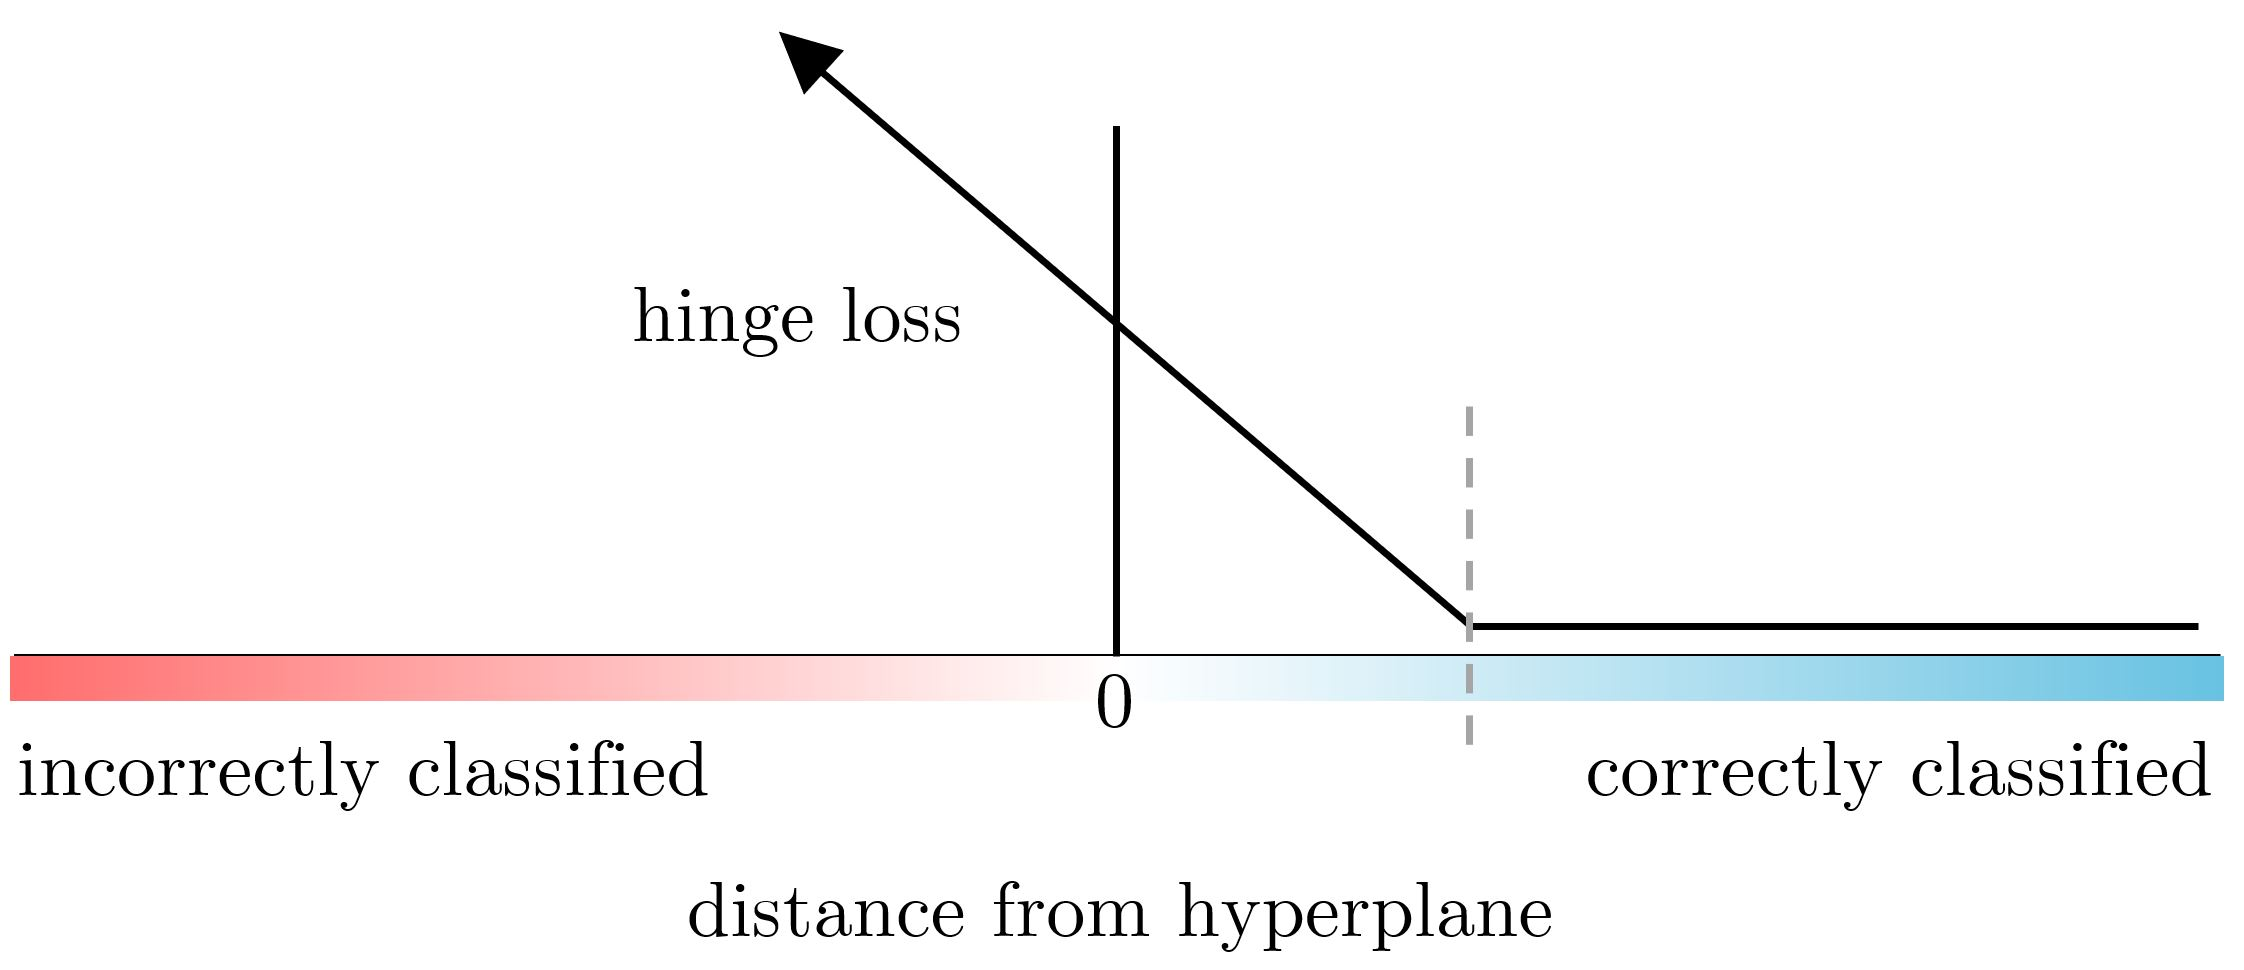
\includegraphics[scale = .105]{images/hingeloss3.JPG}
    \end{center}
    \vspace{-3.5mm}
    \subsection{Multiclass Prediction}
    To classify data with 3$\plus$ classes $C$, a common method is to binarize the problem through:
    \begin{itemize}[label={--},leftmargin=4mm]
        \vspace{-1mm}
        \itemsep -.4mm
        \item One vs. Rest - train a classifier for each class $c_i$ by setting $c_i$'s samples as 1 and all others as 0, and predict the class with the highest confidence score
        \item One vs. One - train $\frac{C (C-1)}{2}$ models for each pair of classes, and predict the class with the highest number of positive predictions
    \end{itemize}

    % ---------------------------------------------------
    \section{k-Nearest Neighbors}
    Non-parametric method that calculates $\hat{y}$ using the average value or most common class of its $k$-nearest points. For high-dimensional data, information is lost through equidistant vectors, so dimension reduction is often applied prior to $k$-NN.

    \textbf{Minkowski Distance} = $(\sum|a_i - b_i|^p)^{1/p}$
    \begin{itemize}[label={--},leftmargin=4mm]
        \itemsep -.4mm
        \item p = 1 gives Manhattan distance ${\sum|a_i - b_i|}$
        \item p = 2 gives Euclidean distance $\sqrt{\sum(a_i - b_i)^2}$
    \end{itemize}

    \textbf{Hamming Distance} - count of the differences between two vectors, often used to compare categorical variables \\

    % \columnbreak
    % ----------------------------------------------------------------
    \textcolor{white}{.}\vspace{-5mm}\\ % Add space above column
    \section{Clustering}
    Unsupervised, non-parametric methods that groups similar data points together based on distance
    \subsection{k-Means}
    Randomly place $k$ centroids across normalized data, and assig observations to the nearest centroid. Recalculate centroids as the mean of assignments and repeat until convergence. Using the median or medoid (actual data point) may be more robust to noise and outliers. $k$-modes is used for categorical data.

    \def\Plus{\texttt{+}}
    $\boldsymbol{k}$\textbf{-means}\Plus\Plus\hspace{1mm}- improves selection of initial clusters
    \begin{enumerate}[leftmargin=5mm]
        \itemsep -.4mm
        \item Pick the first center randomly
        \item Compute distance between points and the nearest center
        \item Choose new center using a weighted probability distribution proportional to distance
        \item Repeat until $k$ centers are chosen
    \end{enumerate}

    Evaluating the number of clusters and performance:

    \textbf{Silhouette Value} - measures how similar a data point is to its own cluster compared to other clusters, and ranges from 1 (best) to -1 (worst).

    \textbf{Davies-Bouldin Index} - ratio of within cluster scatter to between cluster separation, where lower values are better
    % ----------------------------------------------------------------
    \subsection{Hierarchical Clustering}

    Clusters data into groups using a predominant hierarchy

    \textbf{Agglomerative Approach}
    \begin{enumerate}[leftmargin=5mm]
        \itemsep -.4mm
        \item Each observation starts in its own cluster
        \item Iteratively combine the most similar cluster pairs
        \item Continue until all points are in the same cluster
    \end{enumerate}

    \textbf{Divisive Approach} - all points start in one cluster and splits are performed recursively down the hierarchy

    \textbf{Linkage Metrics} - measure dissimilarity between clusters and combines them using the minimum linkage value over all pairwise points in different clusters by comparing:
    \begin{itemize}[label={--},leftmargin=4mm]
        \itemsep -.4mm
        \item Single - the distance between the closest pair of points
        \item Complete - the distance between the farthest pair of points
        \item Ward's - the increase in within-cluster SSE if two clusters were to be combined
    \end{itemize}
    \textbf{Dendrogram} - plots the full hierarchy of clusters, where the height of a node indicates the dissimilarity between its children
    \begin{center}
        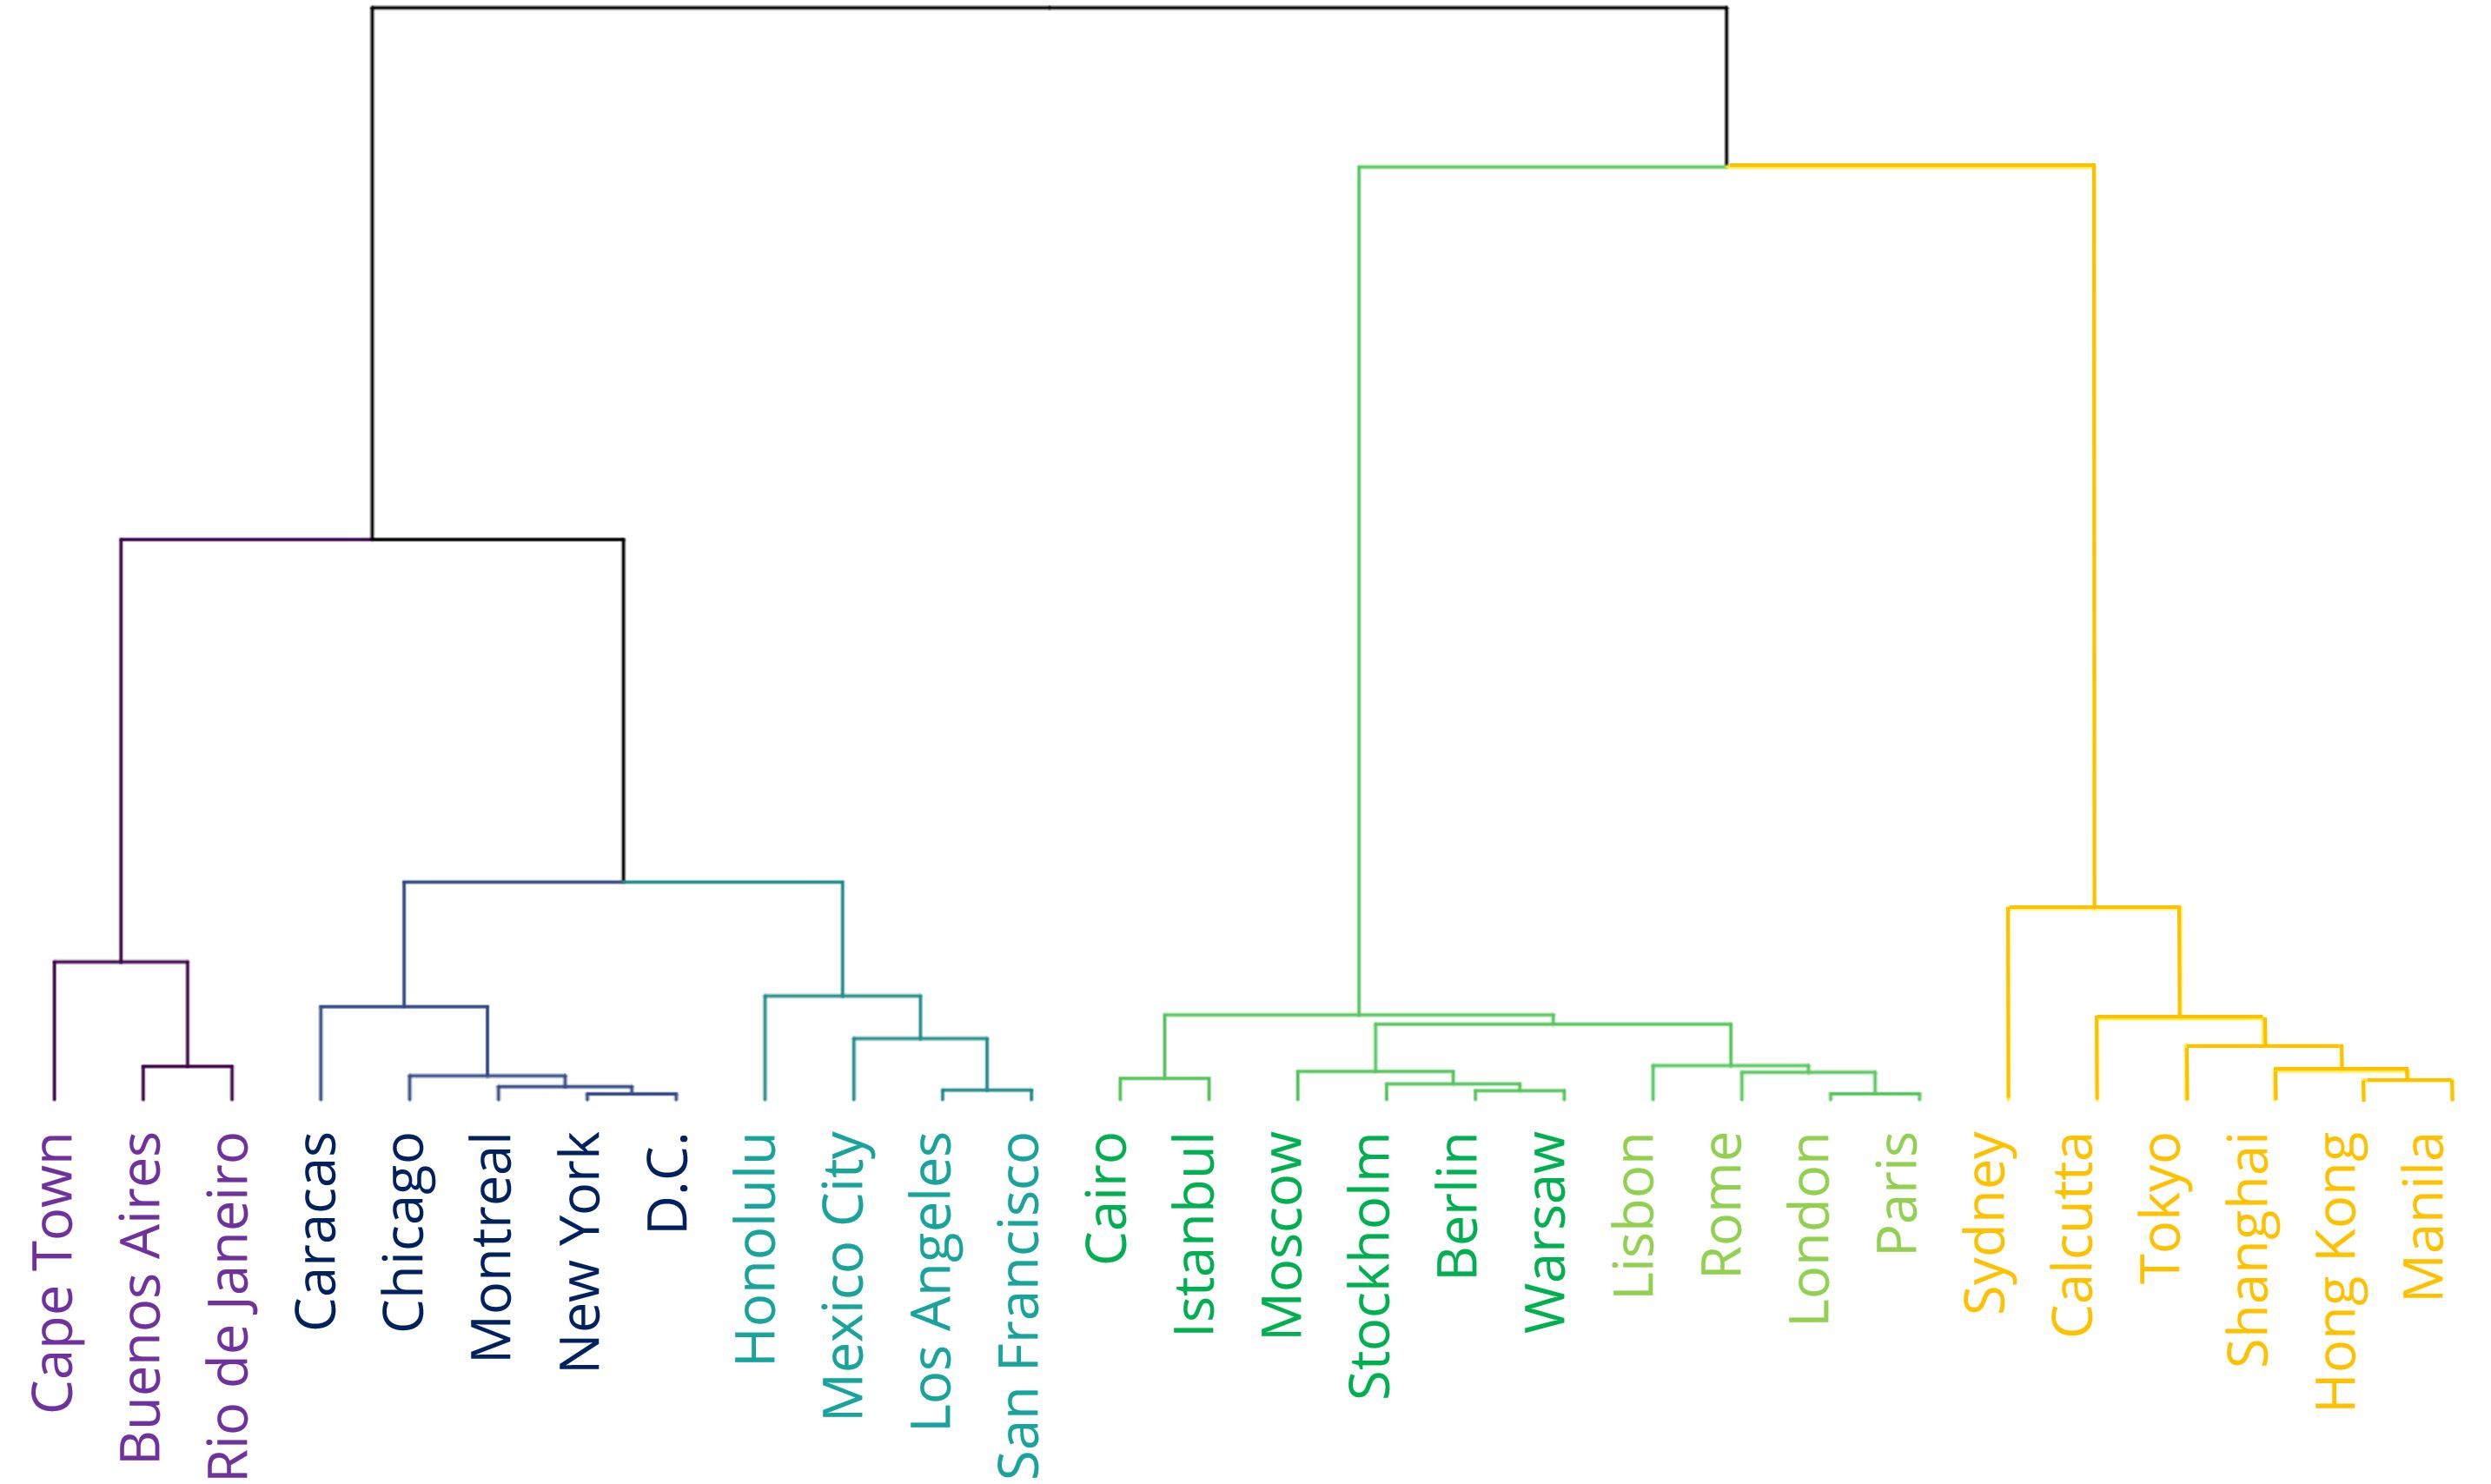
\includegraphics[scale = .1]{images/dendroedit3.JPG}
    \end{center}

    % \columnbreak
    % ----------------------------------------------------------------% ----------------------------------------------------------------
    \textcolor{white}{.}\vspace{-5mm}\\ % Add space above column
    \section{Dimension Reduction}
    High-dimensional data can lead to the \emph{curse of dimensionality}, which increases the risk of overfitting and decreases the value added. The number of samples for each feature combination quickly becomes sparse, reducing model performance.

    \subsection{Principal Component Analysis}
    Projects data onto orthogonal vectors that maximize variance.
    Remember, given an $n\times n$ matrix $A$, a nonzero vector $\vec{x}$, and a scaler $\lambda$, if $A\vec{x} = \lambda \vec{x}$ then $\vec{x}$ and $\lambda$ are an eigenvector and eigenvalue of $A$. In PCA, the eigenvectors are uncorrelated and represent principal components.
    \begin{enumerate}[leftmargin=5mm]
        \itemsep -.4mm
        \item Start with the covariance matrix of standardized data
        \item Calculate eigenvalues and eigenvectors using SVD or eigendecomposition
        \item Rank the principal components by their proportion of variance explained = $\frac{\lambda_i}{\sum{\lambda}}$
    \end{enumerate}

    Data should be linearly related, and for a $p$-dimensional dataset, there will be $p$ principal components.

    Note, PCA explains the variance in X, not necessarily Y.

    \textbf{Sparse PCA} - constrains the number of non-zero values in each component, reducing susceptibility to noise and improving interpretability
    % ----------------------------------------------------------------
    \subsection{Linear Discriminant Analysis}
    Supervised method that maximizes separation between classes and minimizes variance within classes for a labeled dataset
    \begin{enumerate}[leftmargin=5mm]
        \itemsep -.4mm
        \item Compute the mean and variance of each independent variable for every class $C_i$
        \item Calculate the within-class ($\sigma_w^2$) and between-class ($\sigma_b^2$) variance
        \item Find the matrix $W$ = ($\sigma_w^2)^{-1}(\sigma_b^2$) that maximizes Fisher's signal-to-noise ratio
        \item Rank the discriminant components by their signal-to-noise ratio $\lambda$
    \end{enumerate}
    Note, the number of components is at most $C_1 - 1$
    \textbf{Assumptions}
    \vspace{-.7mm}
    \begin{itemize}[label={--},leftmargin=4mm]
        \itemsep -.4mm
        \item Independent variables are normally distributed
        \item Homoscedasticity - constant variance of error
        \item Low multicollinearity
    \end{itemize}


    % ----------------------------------------------------------------
    \subsection{Factor Analysis}
    Describes data using a linear combination of $k$ latent factors.
    Given a normalized matrix $X$, it follows the form  $X = Lf + \epsilon$,  with factor loadings $L$ and hidden factors $f$.
    \vspace{-1mm}
    \begin{center}
        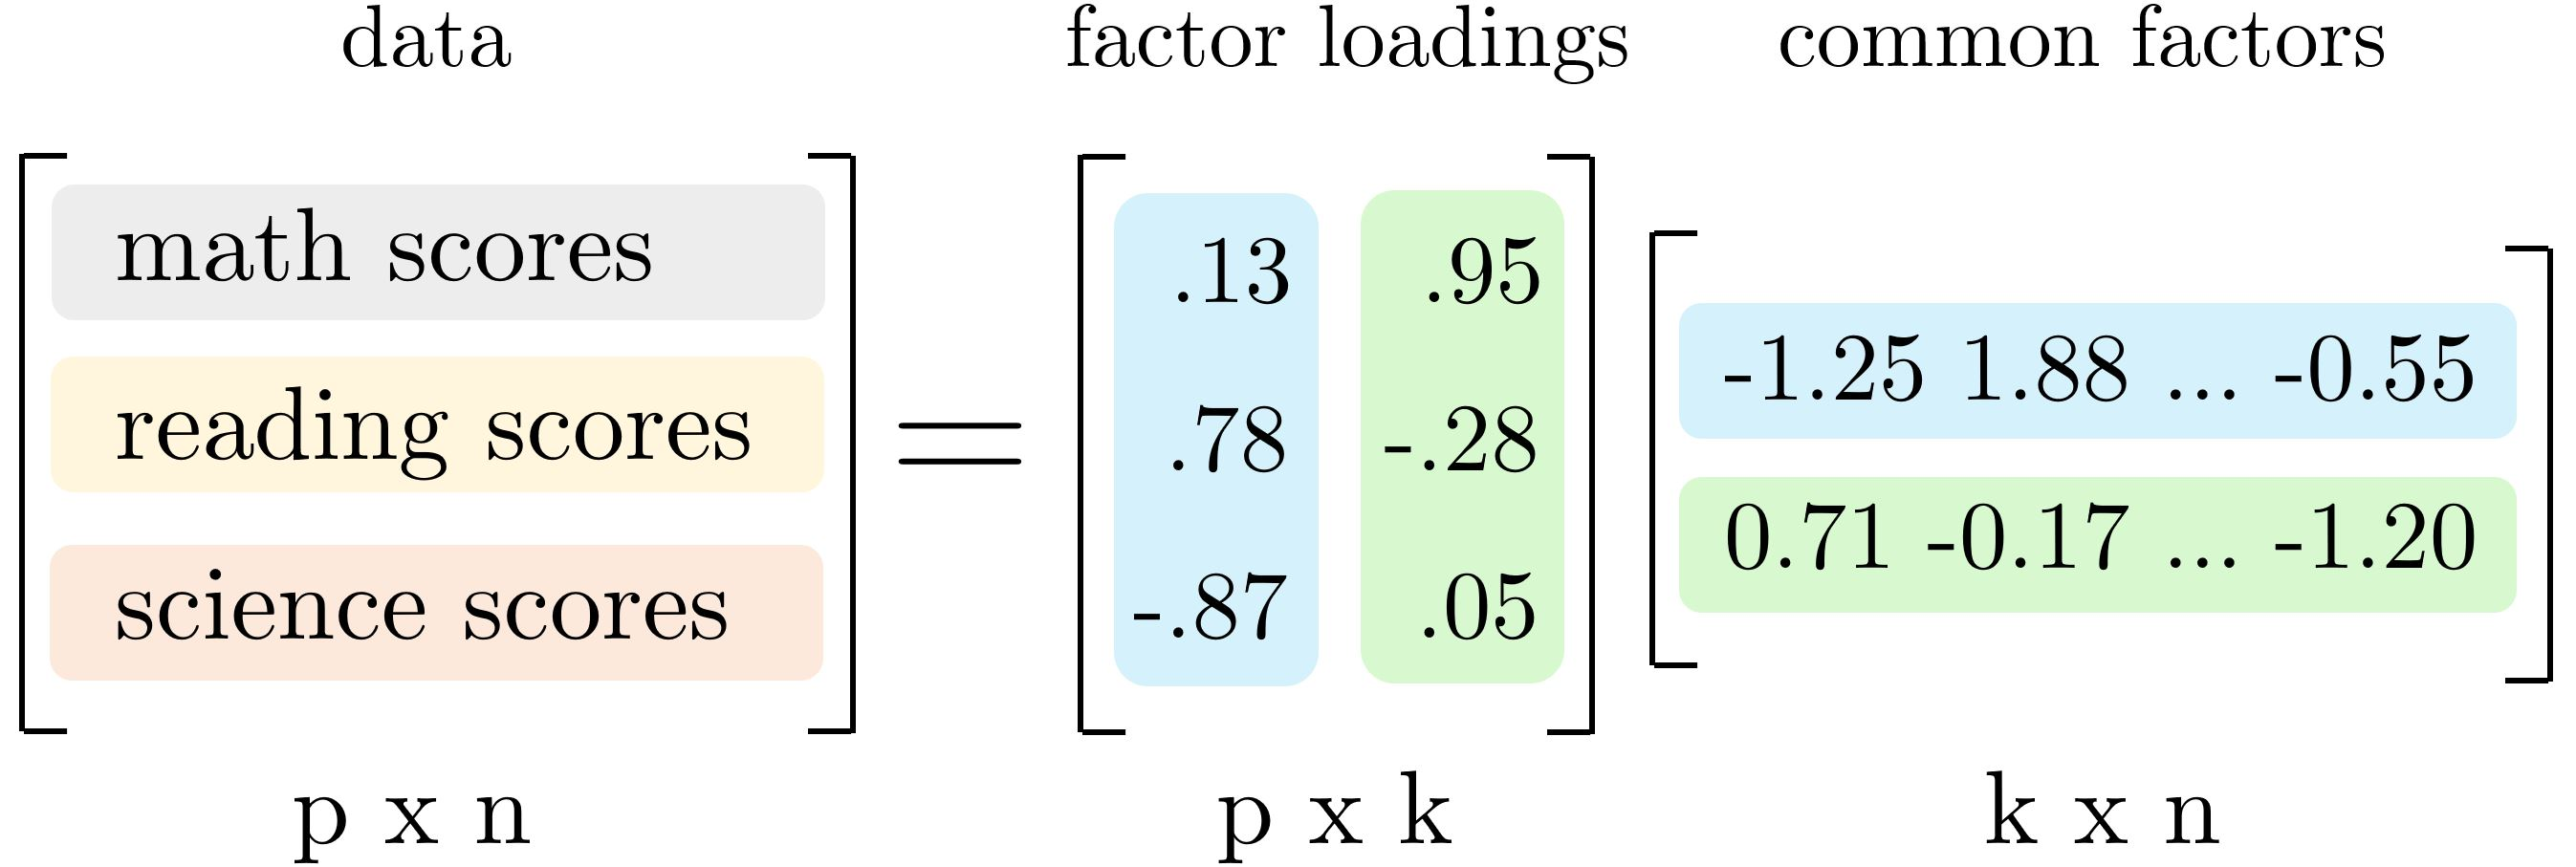
\includegraphics[scale = .1]{images/factorNew1.JPG}
    \end{center}
    \vspace{-2mm}

    \smallskip
    \textbf{Scree Plot} - graphs the eigenvalues of factors (or principal components) and is used to determine the number of factors to retain. The 'elbow' where values level off is often used as the cutoff.
    % \columnbreak
    % ----------------------------------------------------------------
    % ----------------------------------------------------------------
    \\\textcolor{white}{.}\vspace{-5mm}\\ % Add space above column
    \section{Natural Language Processing}
    Transforms human language into machine-usable code
    \textbf{Processing Techniques}
    \begin{itemize}[label={--},leftmargin=4mm]
        \itemsep -.4mm
        \item Tokenization - splits text into individual words (tokens)
        \item Lemmatization - reduces words to its base form based on dictionary definition (\emph{am, are, is} $\to$ \emph{be})
        \item Stemming - reduces words to its base form without context (\emph{ended} $\to$ \emph{end})
        \item Stop words - removes common and irrelevant words (\emph{the, is})
    \end{itemize}

    \textbf{Markov Chain} - stochastic and memoryless process that predicts future events based only on the current state

    $\boldsymbol{n}$\textbf{-gram} - predicts the next term in a sequence of $n$ terms based on Markov chains

    \textbf{Bag-of-words} - represents text using word frequencies, without context or order

    \textbf{tf-idf} - measures word importance for a document in a collection (corpus), by multiplying the term frequency (occurrences of a term in a document) with the inverse document frequency (penalizes common terms across a corpus)
    \textbf{Cosine Similarity} - measures similarity between vectors, calculated as cos($\theta$) =
    $\frac{A\cdot B}{||A||||B||} $, which ranges from o to 1

    \subsection{Word Embedding}
    Maps words and phrases to numerical vectors

    \textbf{word2vec} - trains iteratively over local  word context windows, places similar words close together, and embeds sub-relationships directly into vectors, such that $king - man + woman \approx queen$

    Relies on one of the following:
    \begin{itemize}[label={--},leftmargin=4mm]
        \itemsep -.4mm
        \item Continuous bag-of-words (CBOW) - predicts the word given its context
        \item skip-gram - predicts the context given a word
    \end{itemize}

    \textbf{GloVe} - combines both global and local word co-occurence data to learn word similarity

    \textbf{BERT} - accounts for word order and trains on subwords, and unlike word2vec and GloVe, BERT outputs different vectors for different uses of words ($cell$ phone vs. blood $cell$)

    \subsection{Sentiment Analysis}
    Extracts the attitudes and emotions from text

    \textbf{Polarity} - measures positive, negative, or neutral opinions
    \begin{itemize}[label={--},leftmargin=4mm]
        \itemsep -.4mm
        \item Valence shifters - capture amplifiers or negators such as '$really$ fun' or '$hardly$ fun'
    \end{itemize}
    \textbf{Sentiment} - measures emotional states such as happy or sad
    \textbf{Subject-Object Identification} - classifies sentences as either subjective or objective
    \subsection{Topic Modelling}
    Captures the underlying themes that appear in documents
    \textbf{Latent Dirichlet Allocation} (LDA) - generates $k$ topics by first assigning each word to a random topic, then iteratively updating assignments based on parameters $\alpha$, the mix of topics per document, and $\beta$, the distribution of words per topic

    \textbf{Latent Semantic Analysis} (LSA) - identifies patterns using tf-idf scores and reduces data to $k$ dimensions through SVD
    % \columnbreak

    % -------------------------------------------------------------
    \textcolor{white}{.}\vspace{-5mm}\\ % Add space above column
    \section{Neural Network}
    Feeds inputs through different hidden layers and relies on weights and nonlinear functions to reach an output
    \vspace{-1mm}
    \begin{center}
        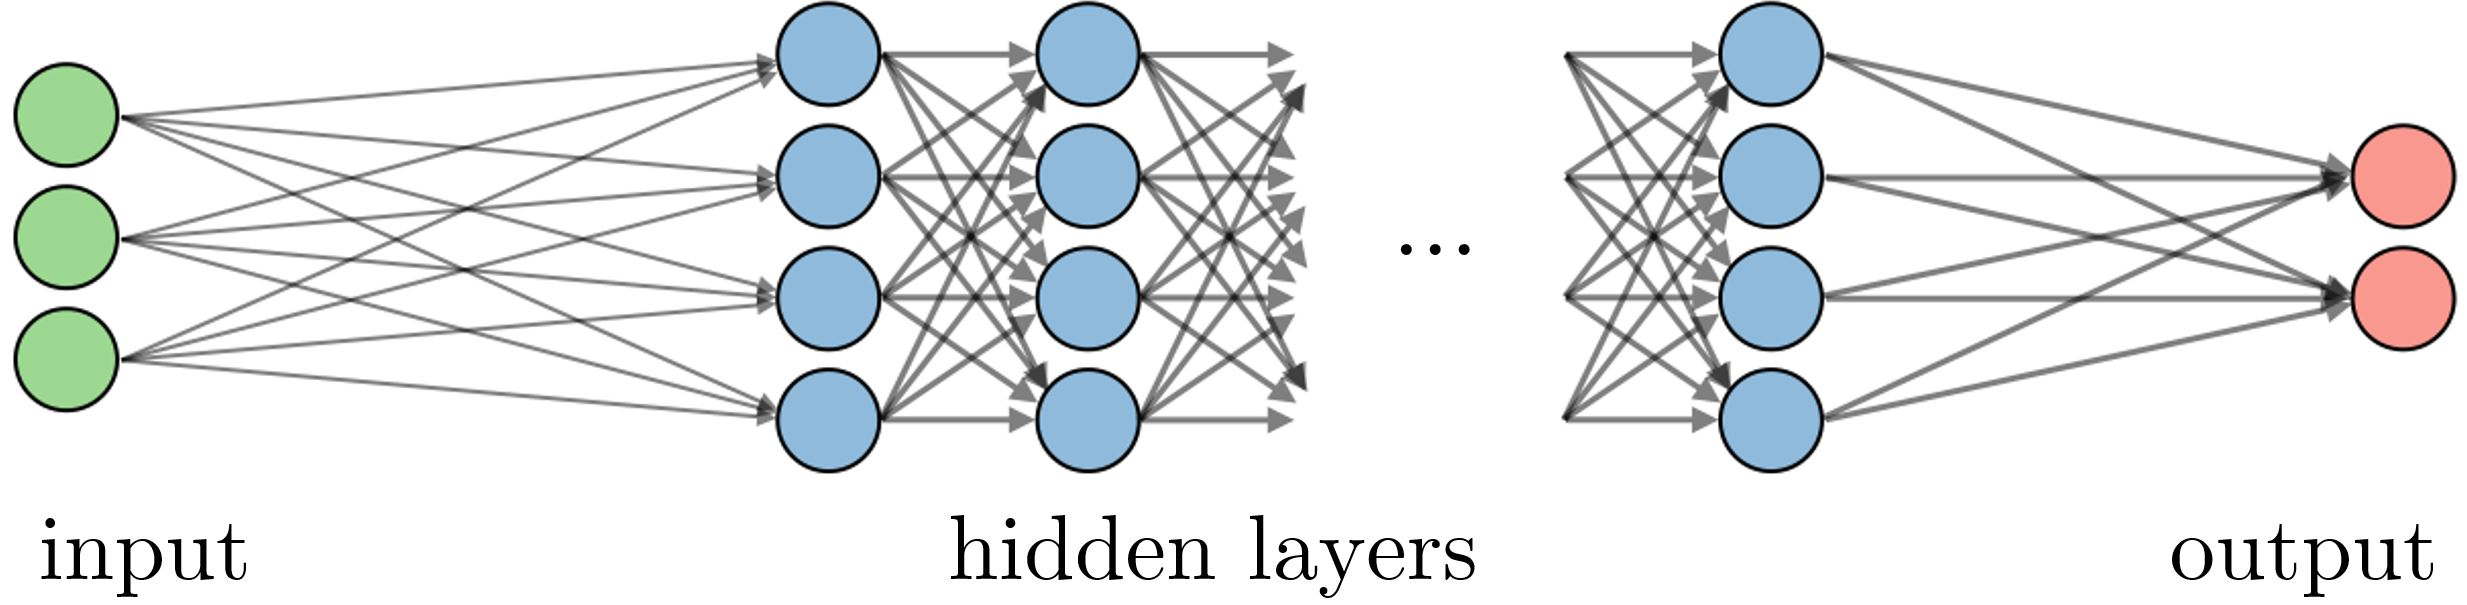
\includegraphics[scale = .11]{images/nn3.JPG}
    \end{center}
    \vspace{-1mm}
    \textbf{Perceptron} - the foundation of a neural network that multiplies inputs by weights, adds bias, and feeds the result $z$ to an activation function

    \textbf{Activation Function} - defines a node's output

    \vspace{-1mm}
    \begin{center}
        \begin{tabular}{c|c|c}
            Sigmoid                                             & ReLU       & Tanh                                \\
            \hline
            \rule{0pt}{3ex}
            $\frac{1}{1+e^{-z}} $                               & max$(0,z)$ & $\frac{e^z - e^{-z}}{e^z + e^{-z}}$ \\
                                                                &            & \vspace{-2mm}                       \\

            \hline
            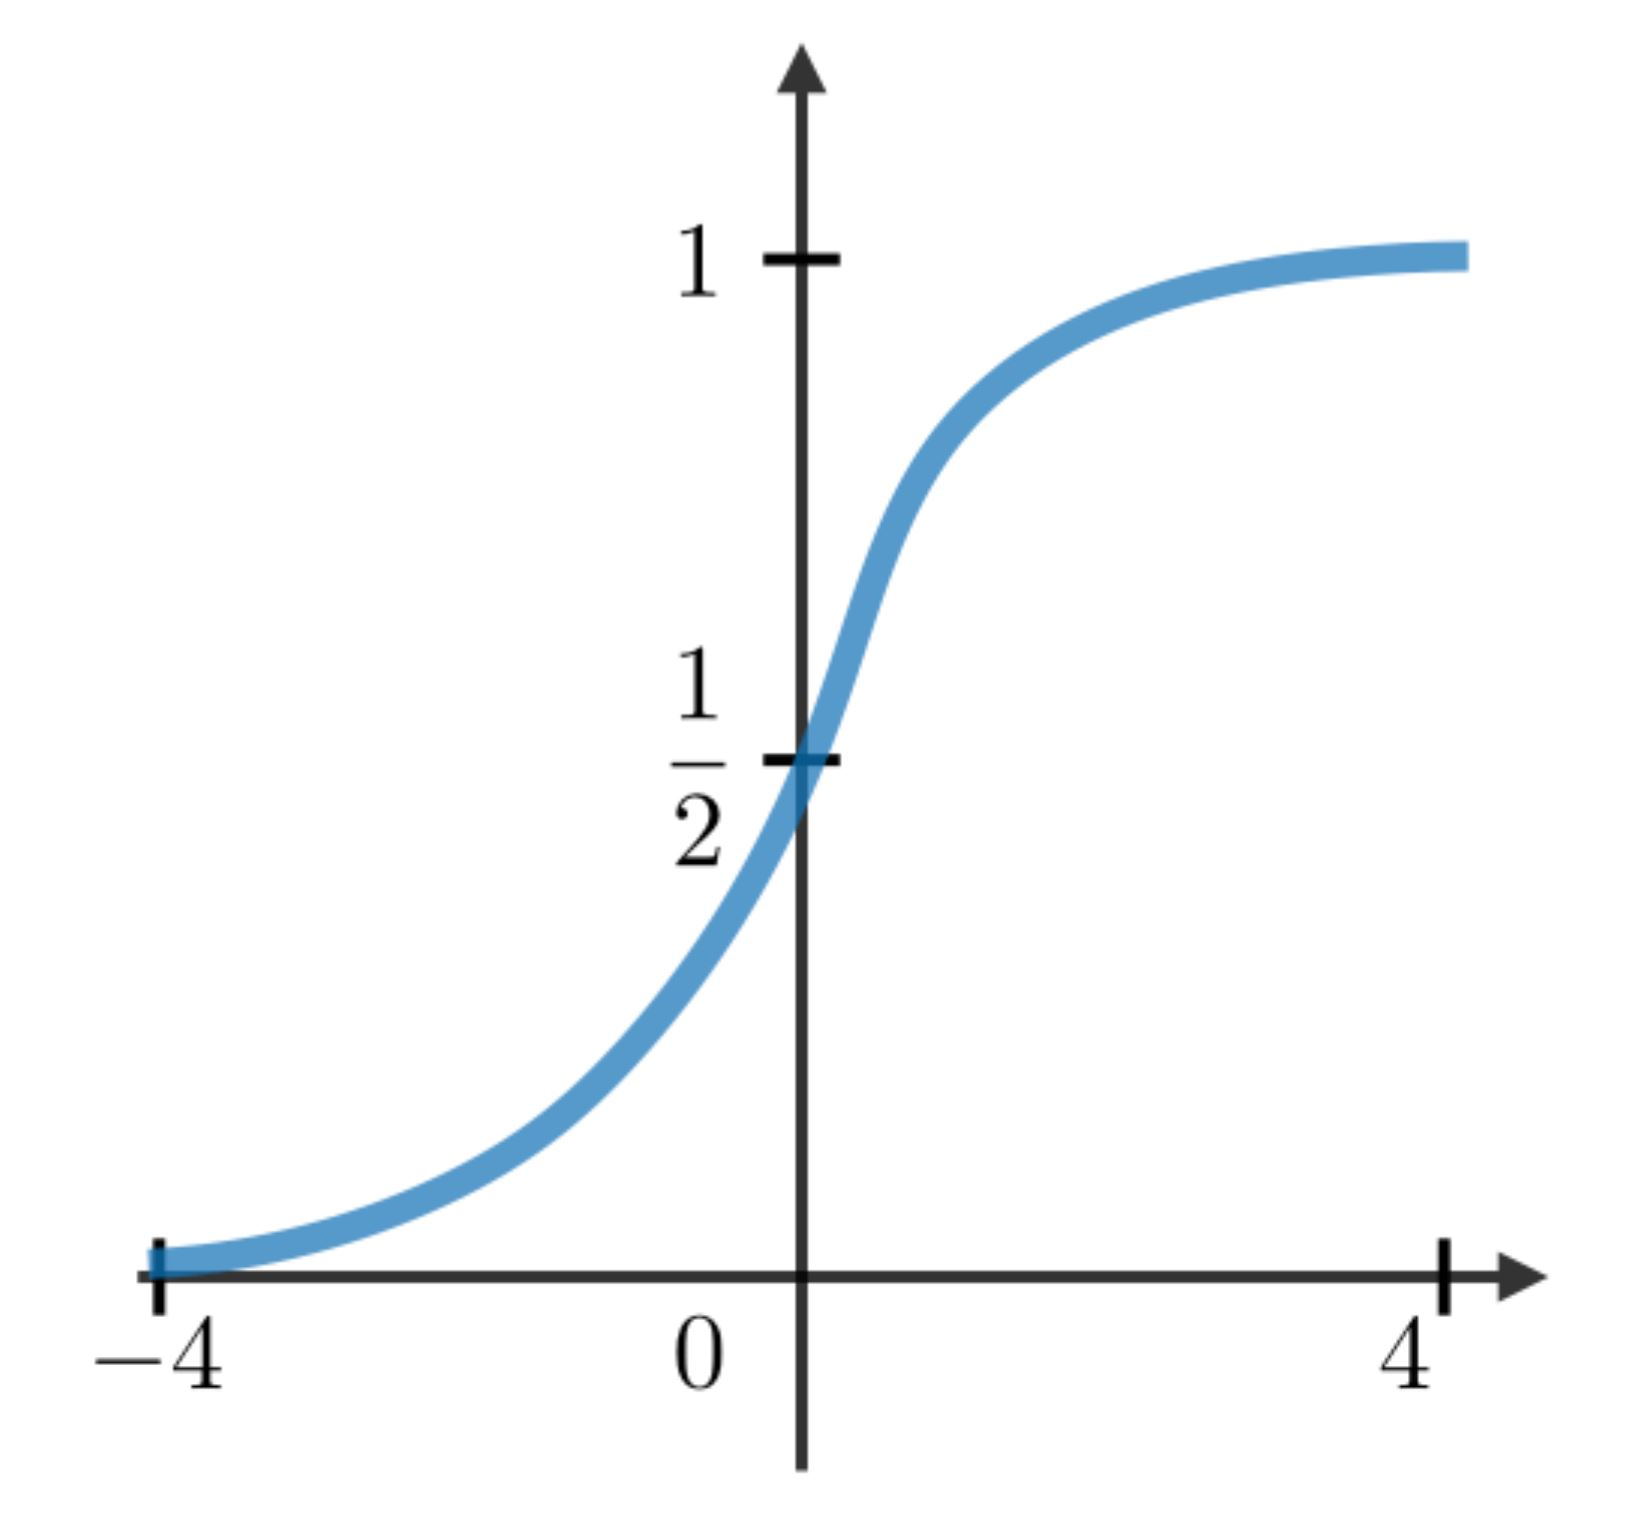
\includegraphics[scale = .047]{images/sigmoid1.JPG} &
            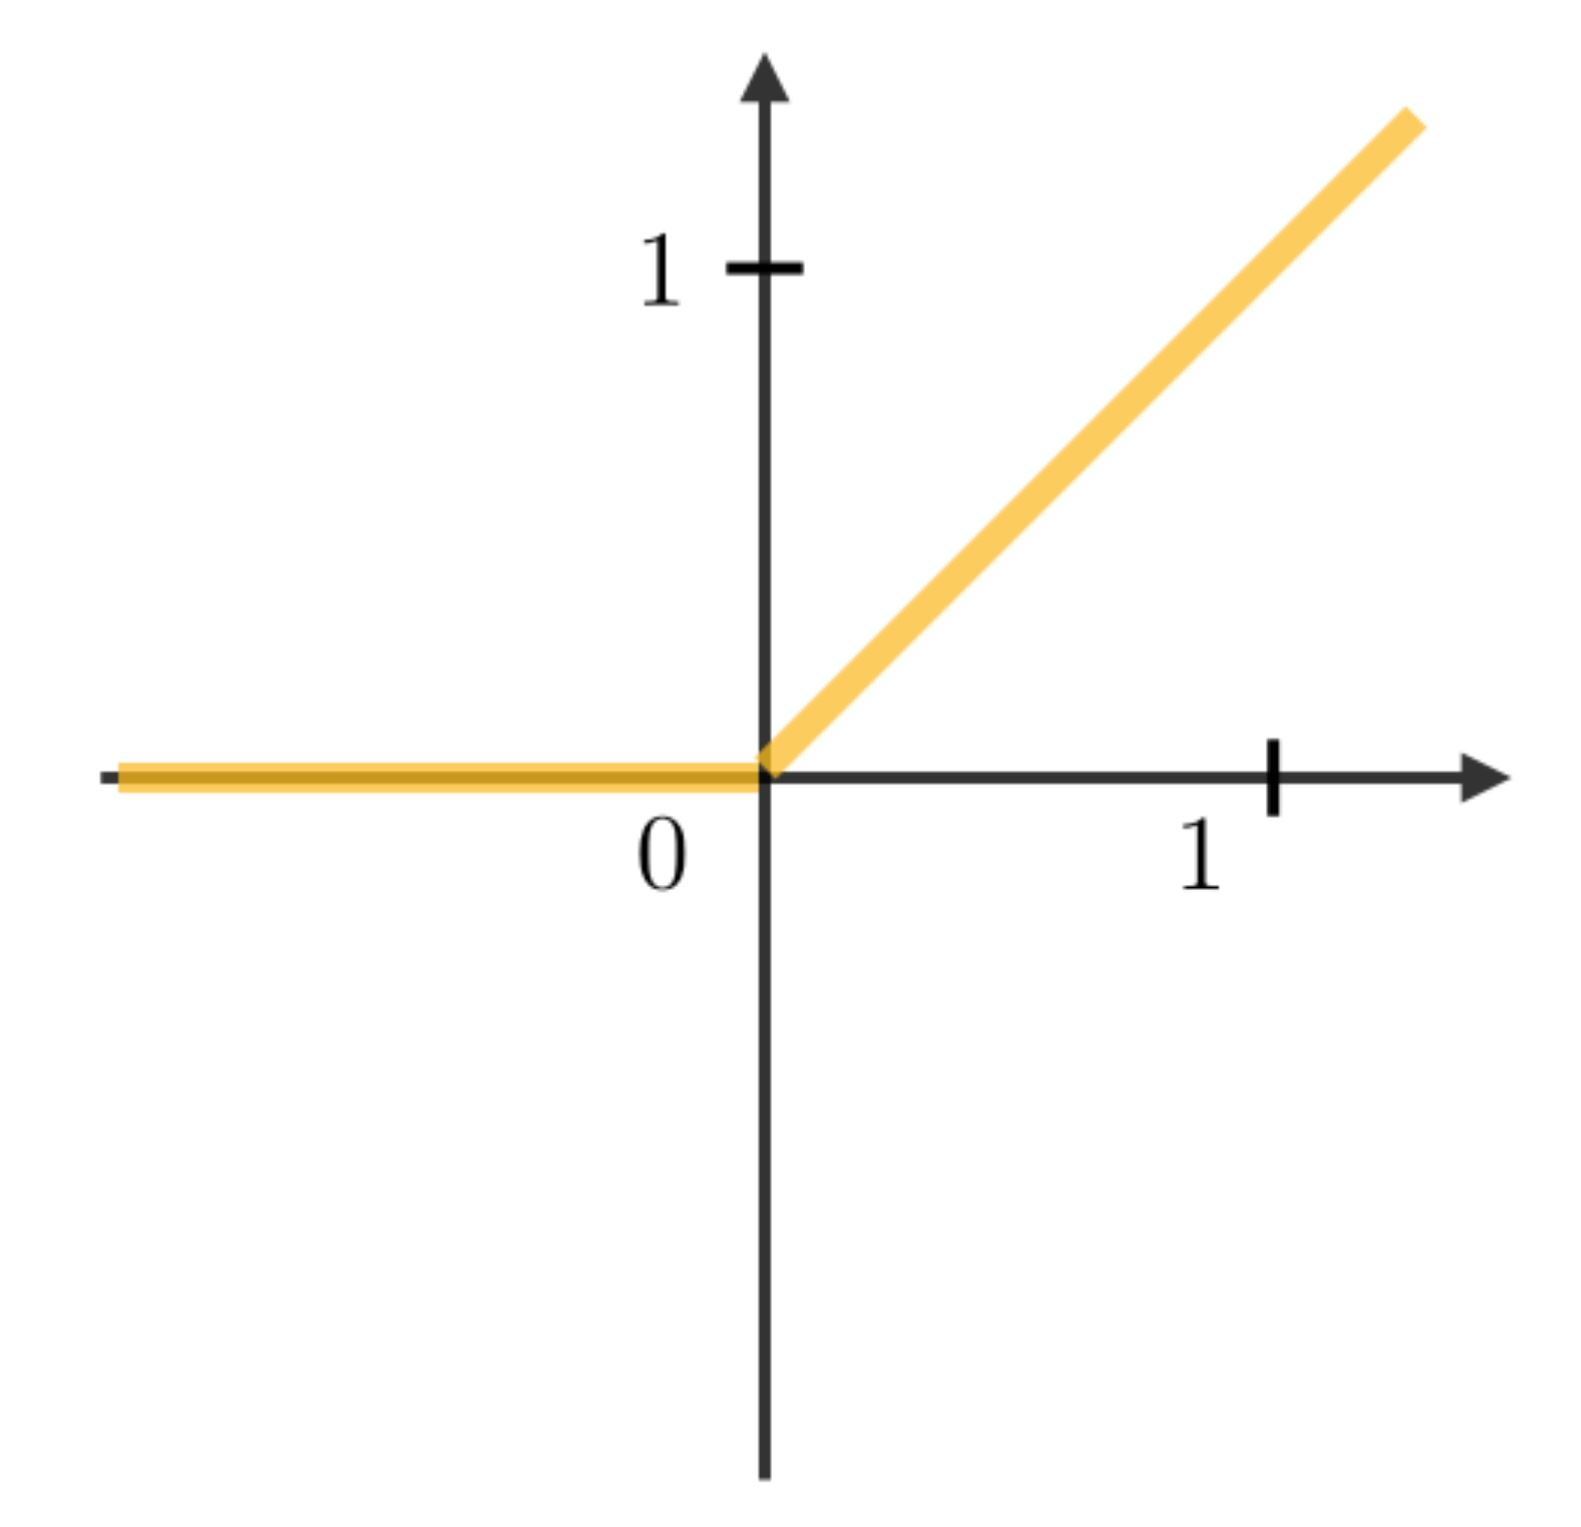
\includegraphics[scale = .047]{images/relu.JPG}     &
            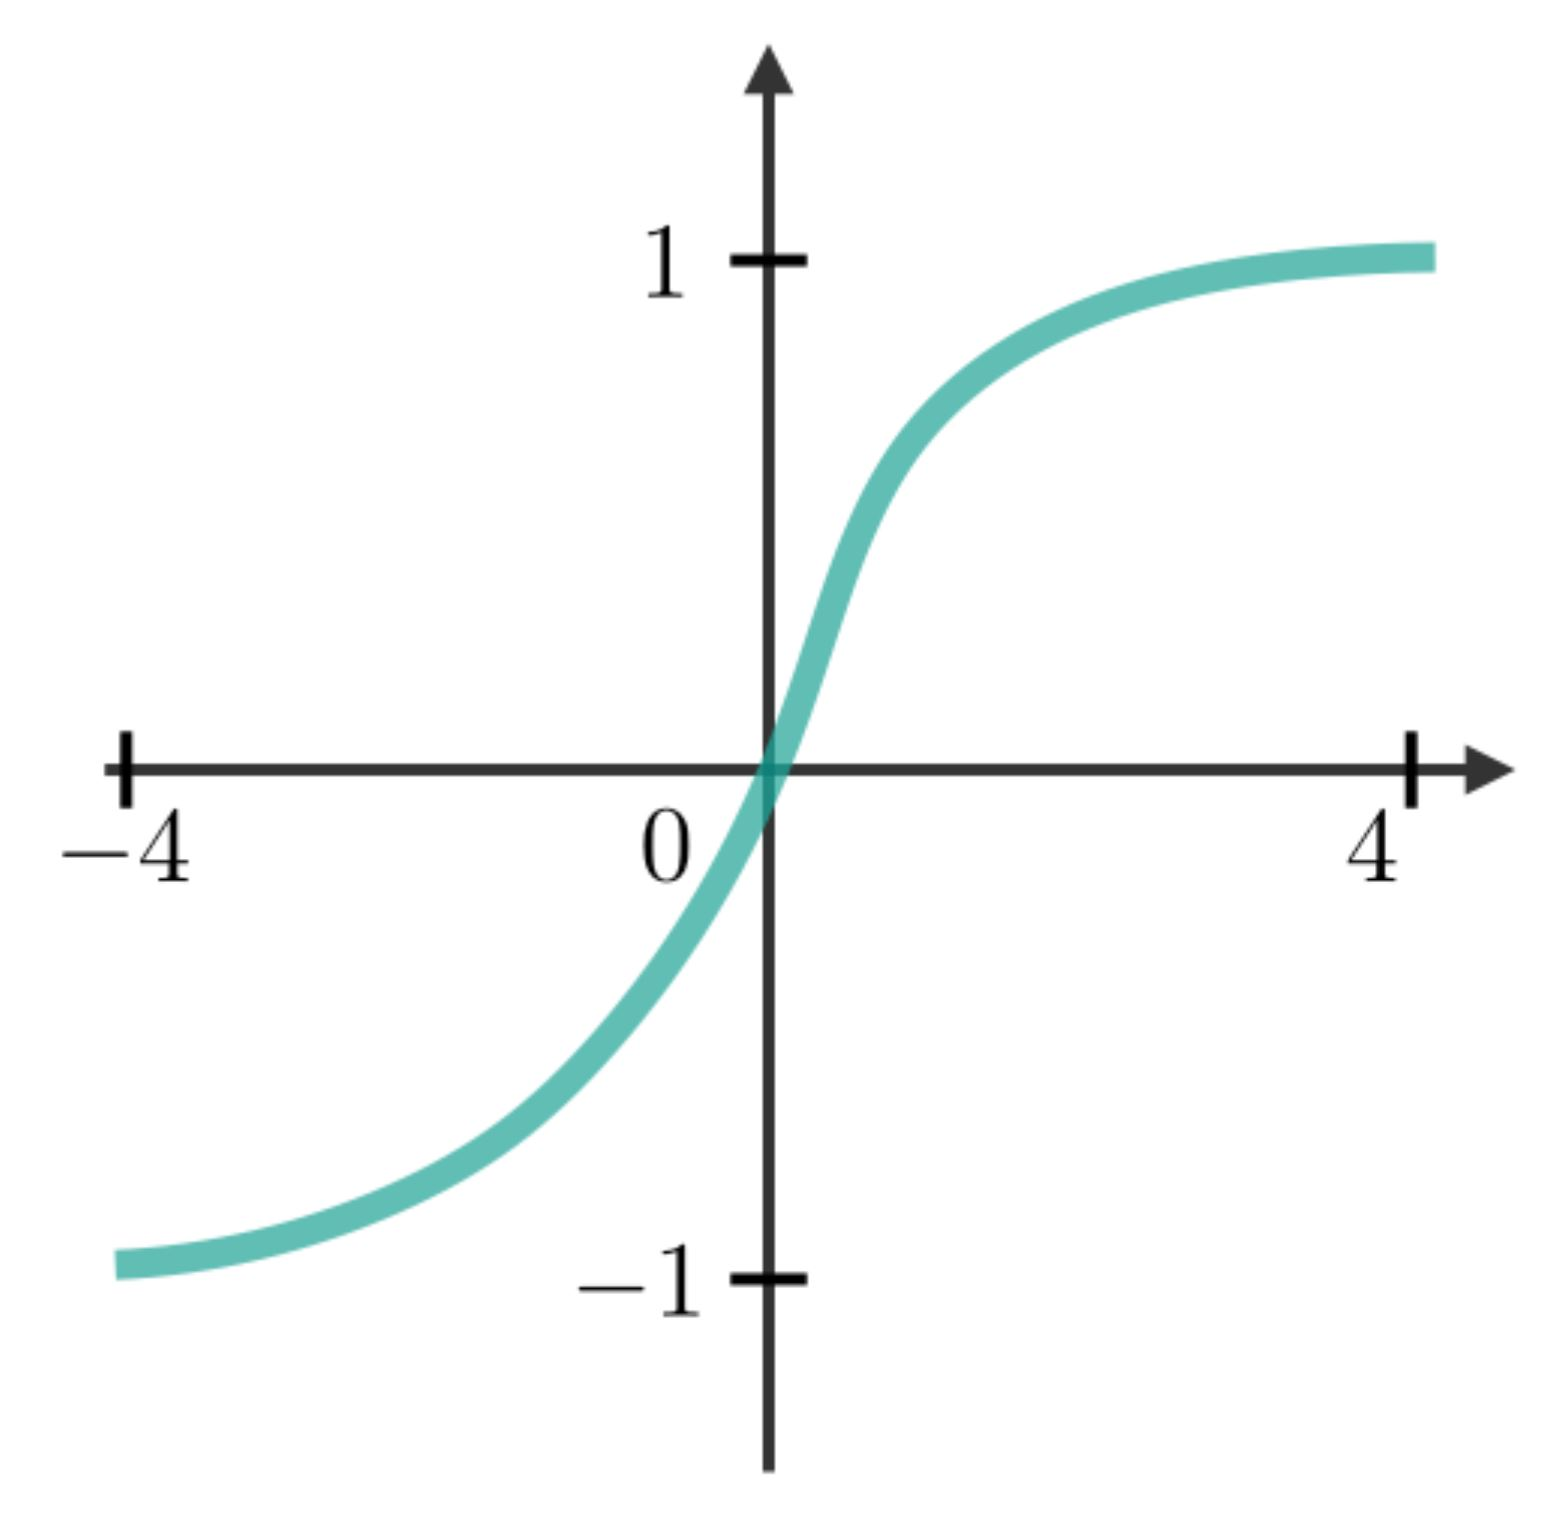
\includegraphics[scale = .047]{images/tanh.JPG}
        \end{tabular}
    \end{center}
    \textbf{Softmax} - given final layer outputs, provides class probabilities that sum to 1 $\to \frac{e^{z_i}}{\sum e^{z}}$

    If there is more than one `correct' label, the sigmoid function provides probabilities for all, some, or none of the labels.


    \smallskip
    \textbf{Loss Function} - measures prediction error using functions such as MSE for regression and binary cross-entropy for probability-based classification

    \smallskip
    \textbf{Gradient Descent} - minimizes the average loss by moving iteratively in the direction of steepest descent, controlled by the learning rate $\gamma$ (step size). Note, $\gamma$ can be updated adaptively for better performance. For neural networks, finding the best set of weights involves:
    \begin{enumerate}[leftmargin=5mm]
        \itemsep -.4mm
        \item Initialize weights $W$ randomly with near-zero values
        \item Loop until convergence:
              \begin{itemize}[label={--},leftmargin=4mm]
                  \itemsep -.4mm
                  \item Calculate the average network loss $J(W)$
                  \item \textbf{Backpropagation} - iterate backwards from the last layer, computing the gradient $\frac{\partial J(W)}{\partial W}$ and updating the weight $W \leftarrow W - \gamma \frac{\partial J(W)}{\partial W}$
              \end{itemize}
        \item Return the minimum loss weight matrix $W$
    \end{enumerate}

    To prevent overfitting, regularization can be applied by:
    \begin{itemize}[label={--},leftmargin=4mm]
        \itemsep -.4mm
        \item Stopping training when validation performance drops
        \item Dropout - randomly drop some nodes during training to prevent over-reliance on a single node
        \item Embedding weight penalties into the objective function
        \item Batch Normalization - stabilizes learning by normalizing inputs to a layer
    \end{itemize}
    \textbf{Stochastic Gradient Descent} - only uses a single point to compute gradients, leading to smoother convergence and faster compute speeds. Alternatively, mini-batch gradient descent trains on small subsets of the data, striking a balance between the approaches.
    \\

    % \columnbreak
    % -------------------------------------------------------------% -------------------------------------------------------------
    \textcolor{white}{.}\vspace{-5mm}\\ % Add space above column
    \section{Convolutional Neural Network}
    Analyzes structural or visual data by extracting local features

    \textbf{Convolutional Layers} - iterate over windows of the image, applying weights, bias, and an activation function to create feature maps. Different weights lead to different features maps.
    \vspace{-4mm}
    \begin{center}
        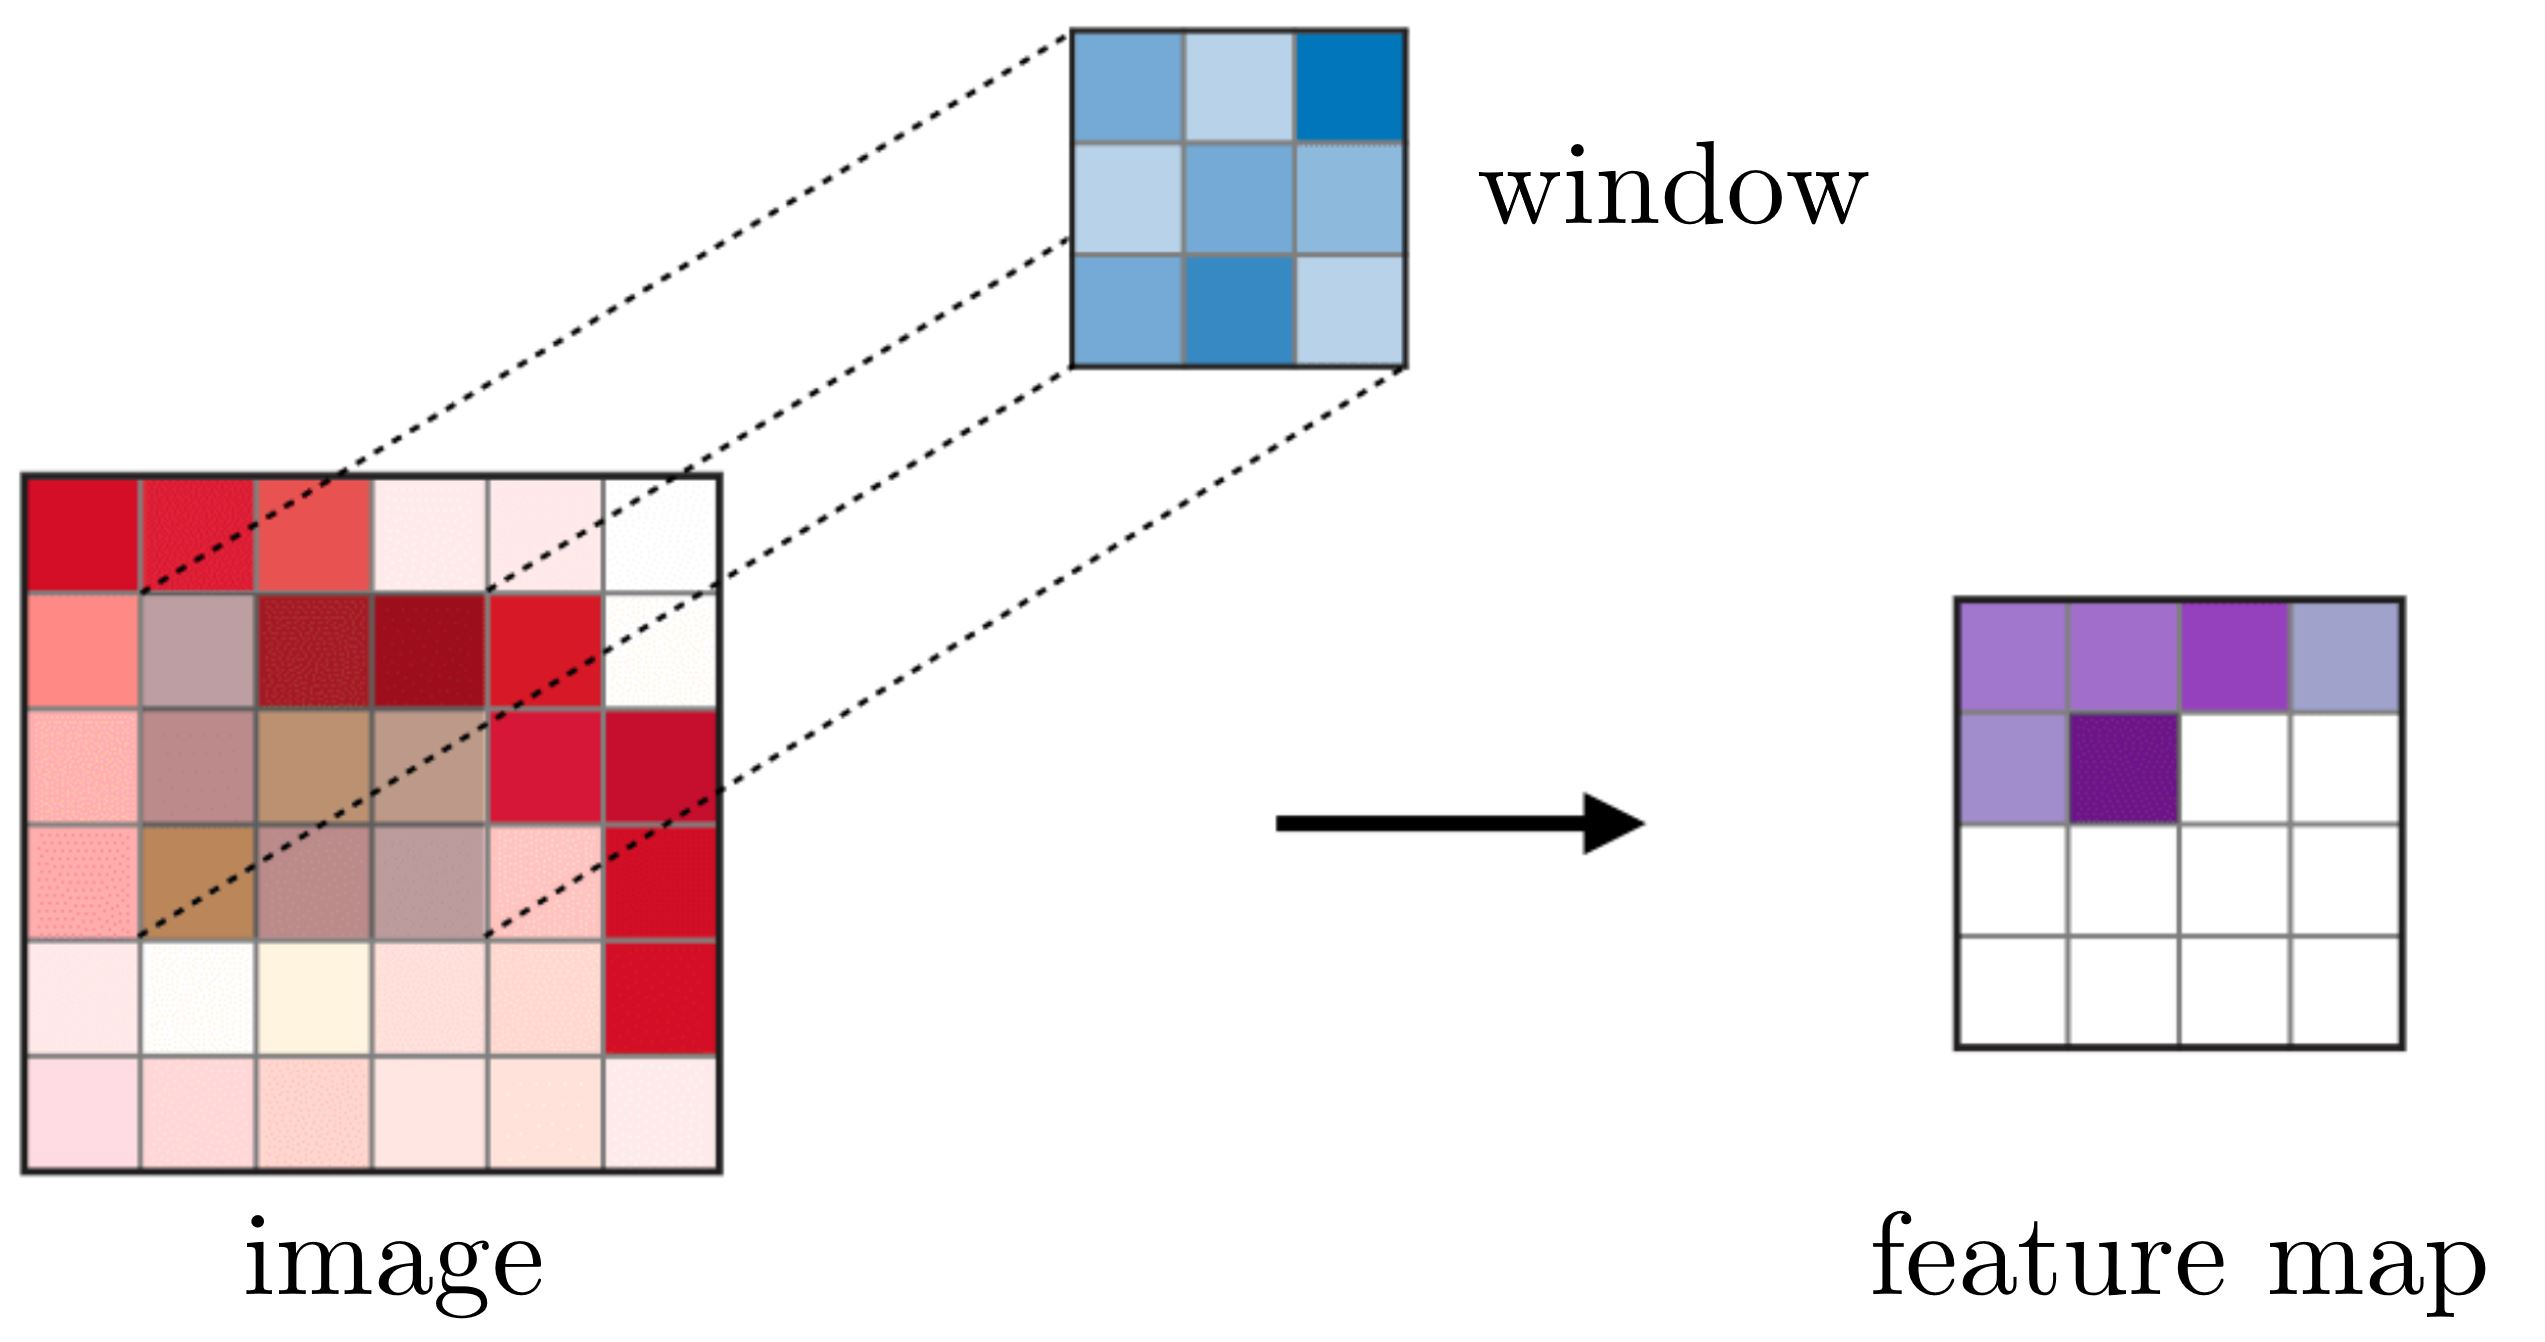
\includegraphics[scale = .06]{images/windowCNNNew.JPG}
    \end{center}
    \vspace{-2mm}
    \textbf{Pooling} - downsamples convolution layers to reduce dimensionality and maintain spatial invariance, allowing detection of features even if they have shifted slightly. Common techniques return the max or average value in the pooling window.\\
    \smallskip
    The general CNN architecture is as follows:
    \begin{enumerate}[leftmargin=5mm]
        \itemsep -.4mm
        \item Perform a series of convolution, ReLU, and pooling operations, extracting important features from the data
        \item Feed output into a fully-connected layer for classification, object detection, or other structural analyses
    \end{enumerate}

    \section{Recurrent Neural Network}
    Predicts sequential data using a temporally connected system that captures both new inputs and previous outputs using hidden states
    \begin{center}
        \vspace{-2mm}
        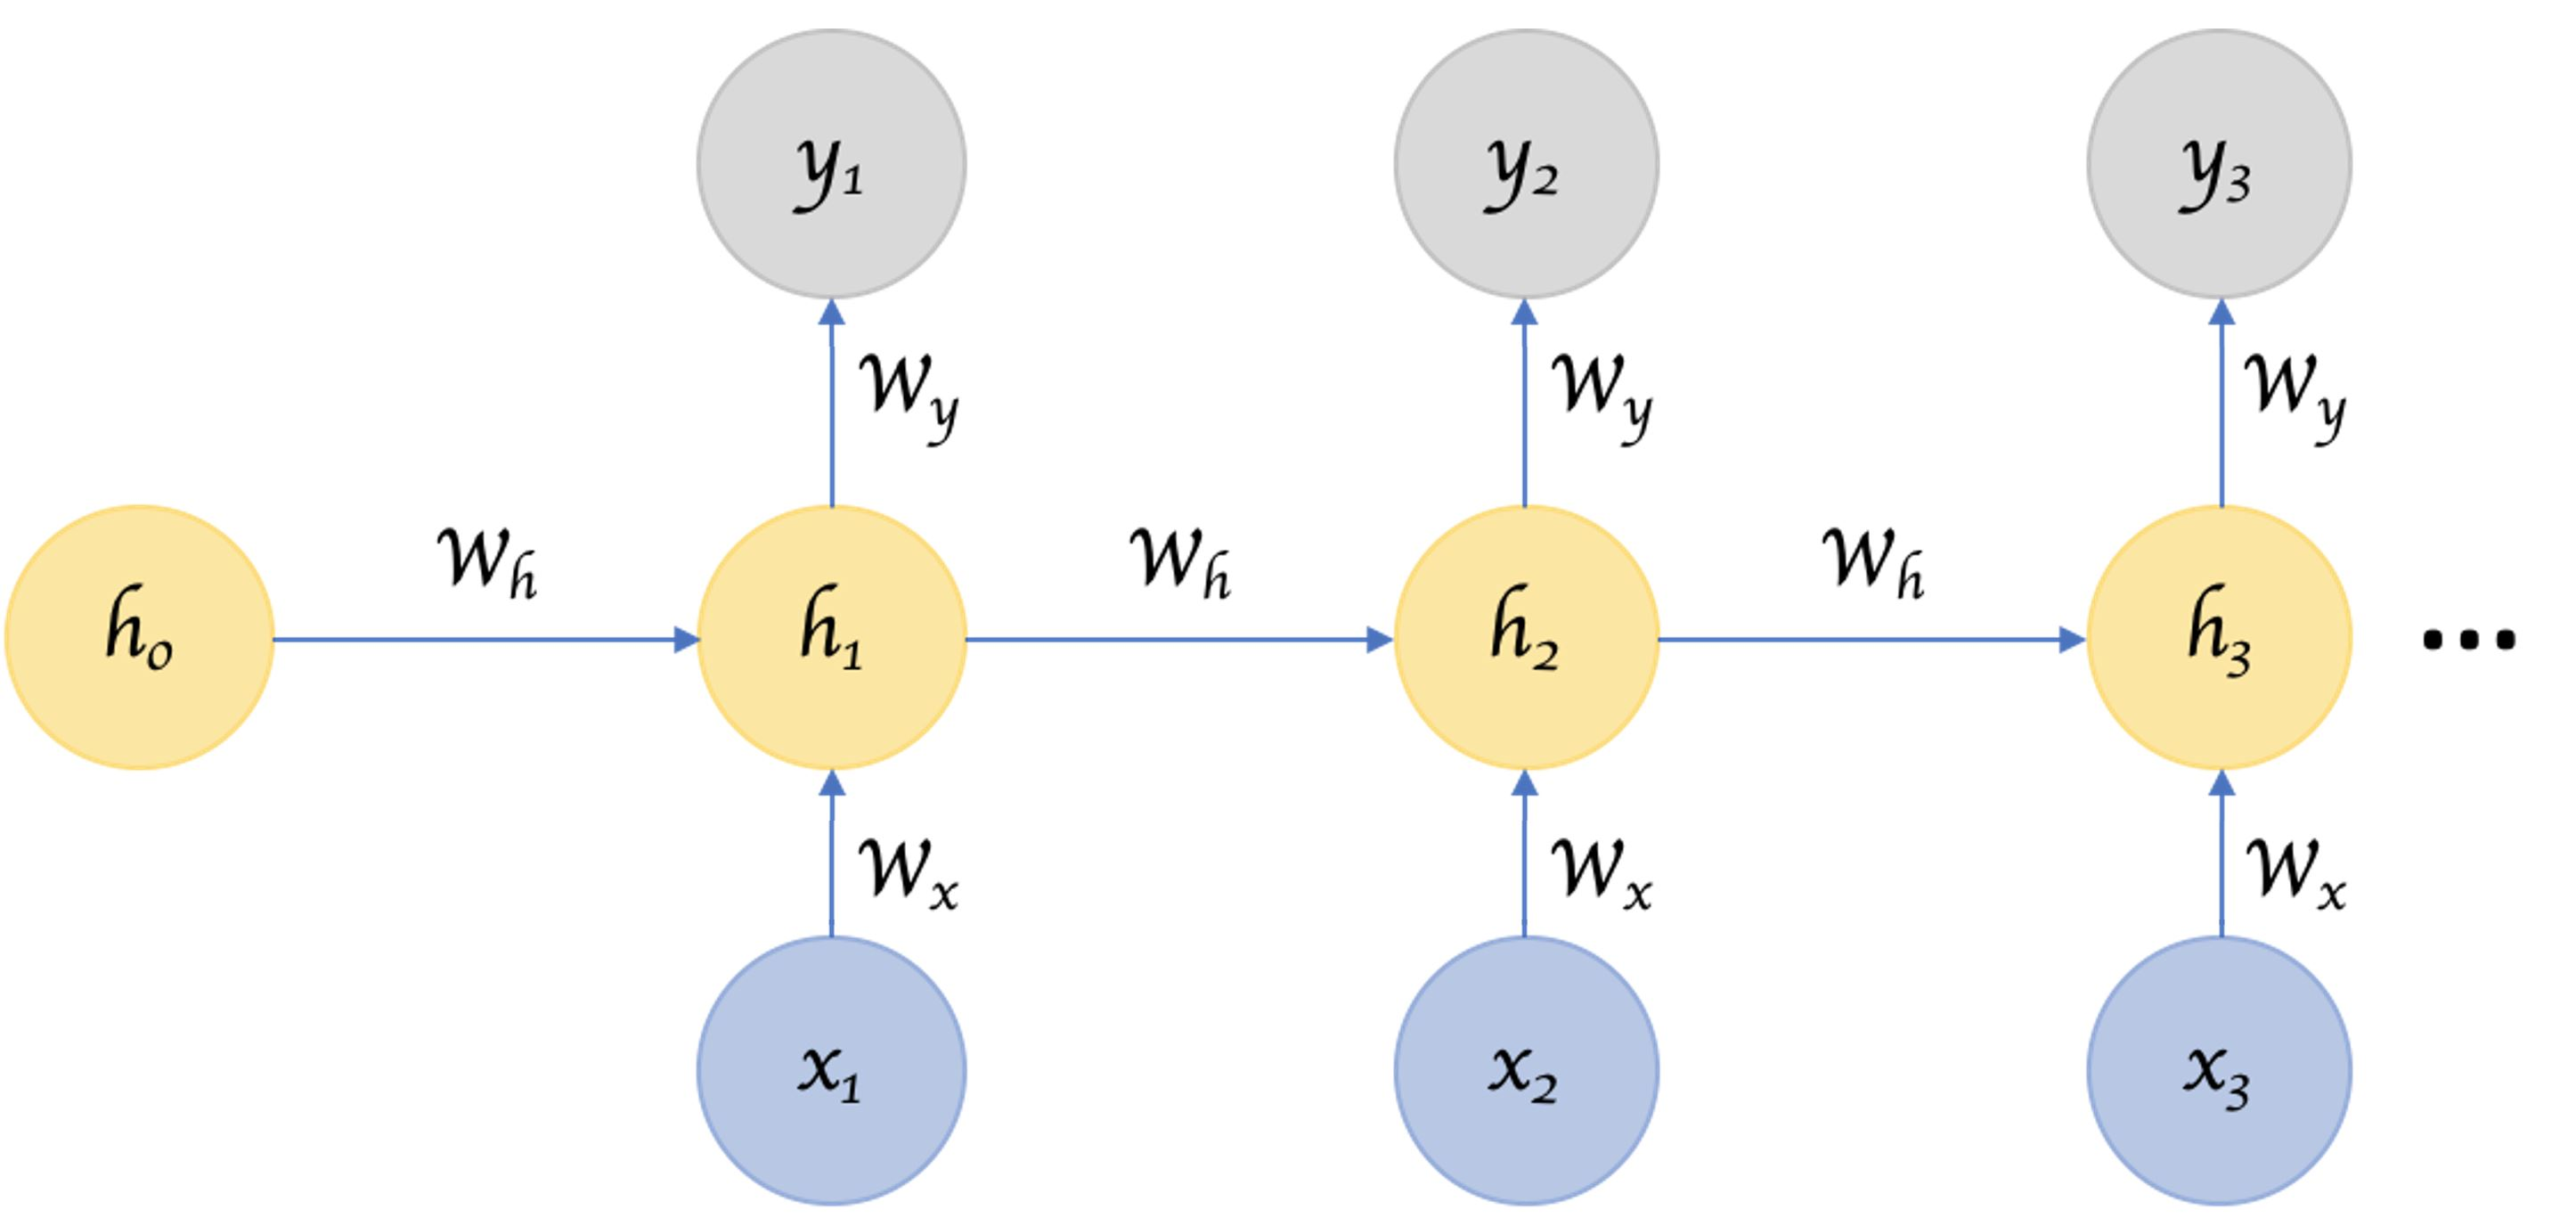
\includegraphics[scale = .07]{images/rnn1.JPG}
    \end{center}
    \vspace{-2mm}

    RNNs can model various input-output scenarios, such as many-to-one, one-to-many, and many-to-many. Relies on parameter (weight) sharing for efficiency. To avoid redundant calculations during backpropagation, downstream gradients are found by chaining previous gradients. However, repeatedly multiplying values greater than or less than 1 leads to:
    \begin{itemize}[label={--},leftmargin=4mm]
        \itemsep -.4mm
        \item Exploding gradients - model instability and overflows
        \item Vanishing gradients - loss of learning ability
    \end{itemize}
    This can be solved using:
    \begin{itemize}[label={--},leftmargin=4mm]
        \itemsep -.4mm
        \item Gradient clipping - cap the maximum value of gradients
        \item ReLU - its derivative prevents gradient shrinkage for $x > 0$
        \item Gated cells - regulate the flow of information
    \end{itemize}

    \textbf{Long Short-Term Memory} - learns long-term dependencies using gated cells and maintains a separate cell state from what is outputted. Gates in LSTM perform the following:

    \begin{enumerate}[leftmargin=5mm]
        \itemsep -.4mm
        \item Forget and filter out irrelevant info from previous layers
        \item Store relevant info from current input
        \item Update the current cell state
        \item Output the hidden state, a filtered version of the cell state
    \end{enumerate}
    LSTMs can be stacked to improve performance.

    % \columnbreak
    % -------------------------------------------------------------% -------------------------------------------------------------
    \textcolor{white}{.}\vspace{-3mm}\\ % Add space above column
    \section{Attention and Transformers}
    \section{Boosting}
    Sequentially fits many simple models that account for the previous model's errors. As opposed to bagging, boosting trains on all the data and combines models using the learning rate $\alpha$. \\
    \smallskip
    \textbf{AdaBoost} - uses sample weighting and decision 'stumps' (one-level decision trees) to classify samples
    \begin{enumerate}[leftmargin=5mm]
        \itemsep -.4mm
        \item Build decision stumps for every feature, choosing the one with the best classification accuracy
        \item Assign more weight to misclassified samples and reward trees that differentiate them, where  $\alpha = \frac{1}{2}ln\frac{1-TotalError}{TotalError}$
        \item Continue training and weighting decision stumps until convergence
    \end{enumerate}

    \textbf{Gradient Boost} - trains sequential models by minimizing a given loss function using gradient descent at each step
    \begin{enumerate}[leftmargin=5mm]
        \itemsep -.4mm
        \item Start by predicting the average value of the response
        \item Build a tree on the errors, constrained by depth or the number of leaf nodes
        \item Scale decision trees by a constant learning rate $\alpha$
        \item Continue training and weighting decision trees until convergence
    \end{enumerate}

    XGBoost - fast gradient boosting method that utilizes regularization and parallelization
    % -------------------------------------------------------------% -------------------------------------------------------------
    \section{Recommender Systems}
    Suggests relevant items to users by predicting ratings and preferences, and is divided into two main types:
    \begin{itemize}[label={--},leftmargin=4mm]
        \itemsep -.4mm
        \item Content Filtering - recommends similar items
        \item Collaborative Filtering - recommends what similar users like
    \end{itemize}

    The latter is more common, and includes methods such as:
    \textbf{Memory-based Approaches} - finds neighborhoods by using rating data to compute user and item similarity, measured using correlation or cosine similarity

    \begin{itemize}[label={--},leftmargin=4mm]
        \itemsep -.4mm
        \item User-User - similar users also liked...
              \begin{itemize}[label={--},leftmargin=4mm]
                  \vspace{-1mm}
                  \itemsep -.4mm
                  \item Leads to more diverse recommendations, as opposed to just recommending popular items
                  \item Suffers from sparsity, as the number of users who rate items is often low
              \end{itemize}
              \vspace{-1mm}
        \item Item-Item - similar users who liked this item also liked...
              \begin{itemize}[label={--},leftmargin=4mm]
                  \itemsep -.4mm
                        \vspace{-1.5mm}
                  \item Efficient when there are more users than items, since the item neighborhoods update less frequently than users
                  \item Similarity between items is often more reliable than similarity between users
              \end{itemize}
    \end{itemize}
    \vspace{-1.5mm}
    \smallskip
    \textbf{Model-based Approaches} - predict ratings of unrated items, through methods such as Bayesian networks, SVD, and clustering. Handles sparse data better than memory-based approaches.\\
    \begin{itemize}[label={--},leftmargin=4mm]
        \itemsep -.4mm
              \vspace{-.5mm}
        \item Matrix Factorization - decomposes the user-item rating matrix into two lower-dimensional matrices representing the users and items, each with $k$ latent factors
    \end{itemize}
    \smallskip
    \vspace{-1mm}
    Recommender systems can also be combined through ensemble methods to improve performance.
    % \columnbreak
    % -------------------------------------------------------------% -------------------------------------------------------------
    \\\textcolor{white}{.}\vspace{-3mm}\\ % Add space above column
    \section{Reinforcement Learning}
    Maximizes future rewards by learning through state-action pairs. That is, an $agent$ performs $actions$ in an $environment$, which updates the $state$ and provides a $reward$.

    \begin{center}
        \vspace{-2mm}
        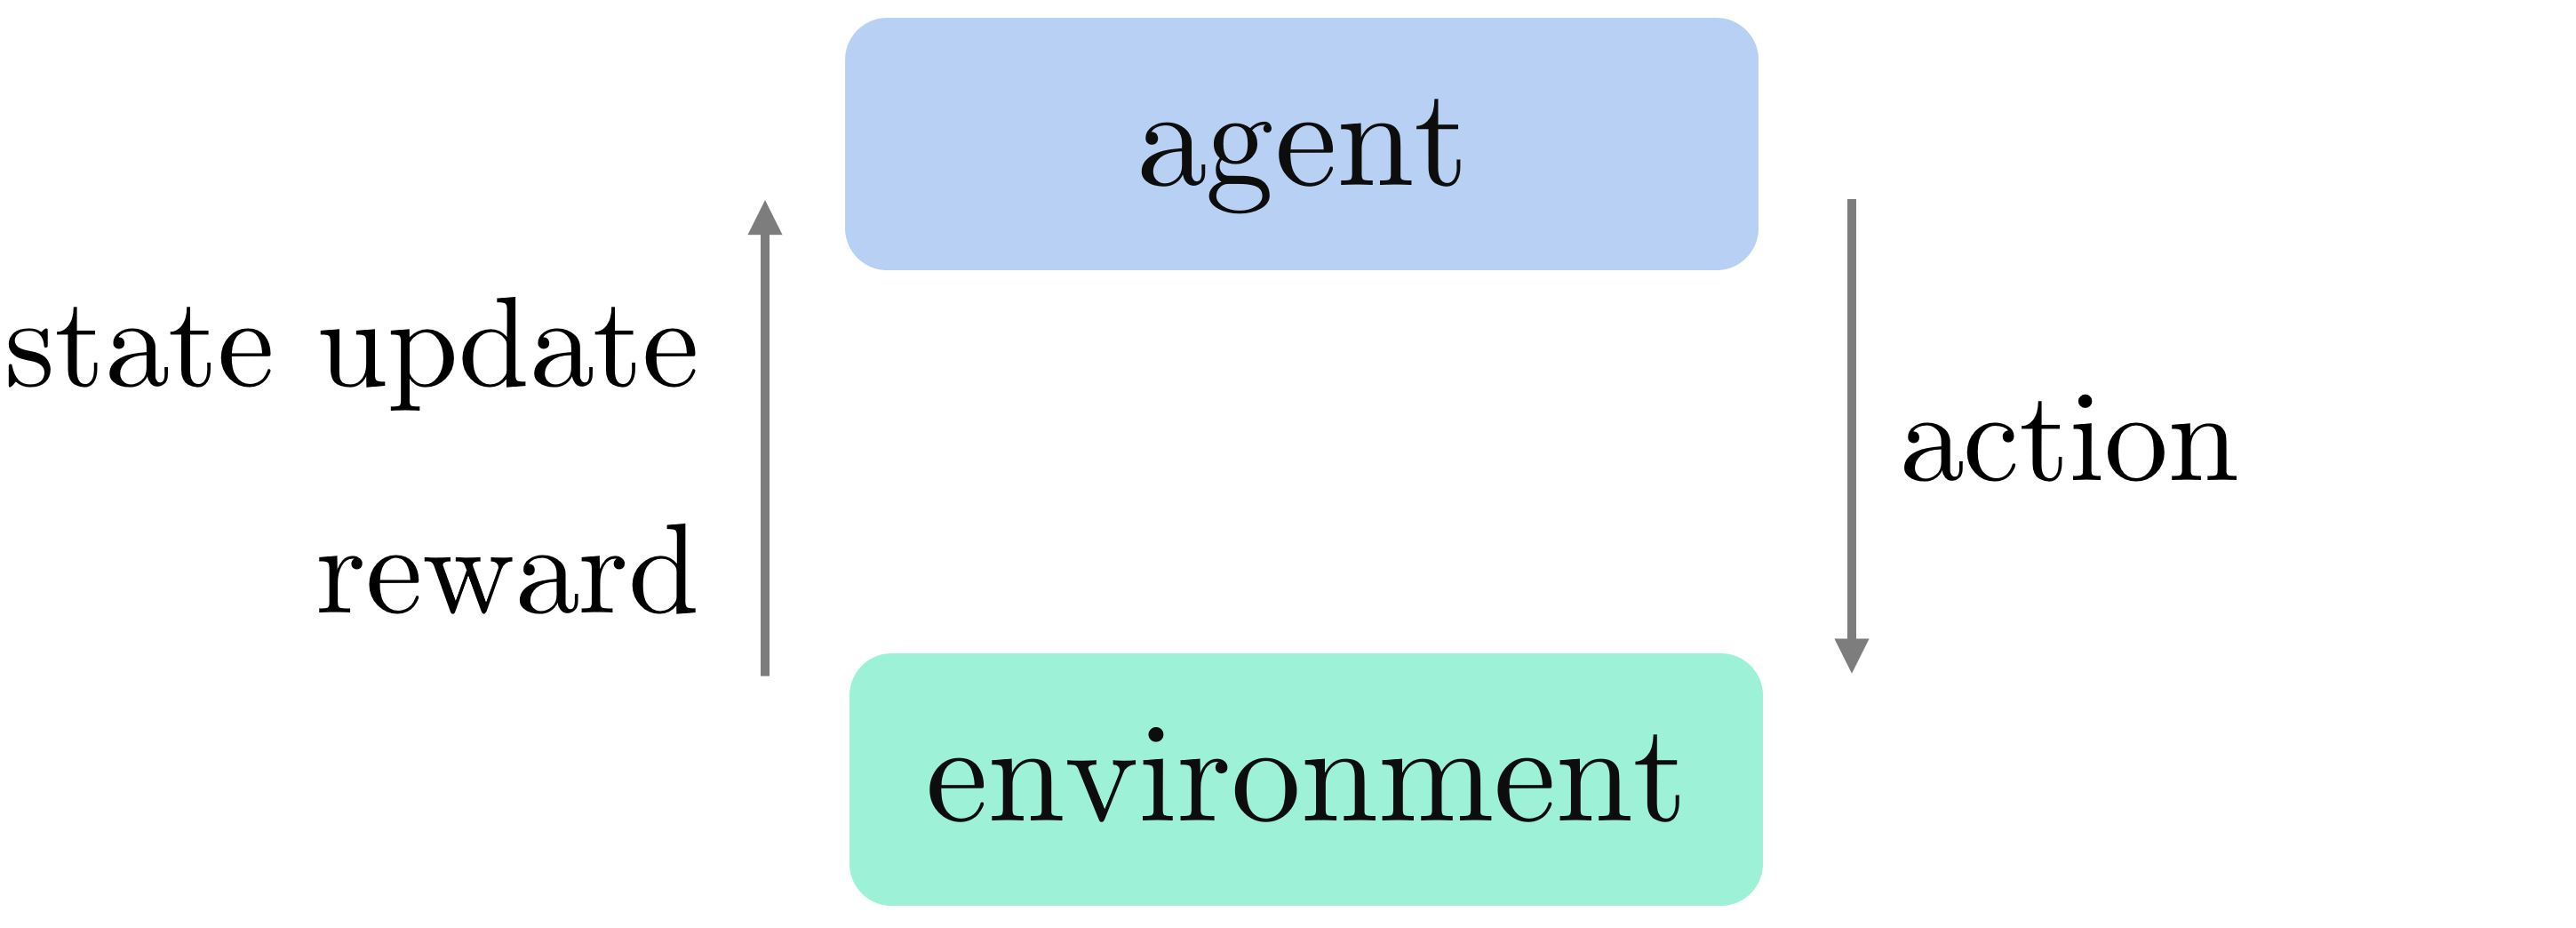
\includegraphics[scale = .085]{images/reinforcement4.JPG}
    \end{center}
    \vspace{-2.5mm}
    \textbf{Multi-armed Bandit Problem} - a gambler plays slot machines with unknown probability distributions and must decide the best strategy to maximize reward. This exemplifies the exploration-exploitation tradeoff, as the best long-term strategy may involve short-term sacrifices.\\
    \smallskip
    RL is divided into two types, with the former being more common:
    \begin{itemize}[label={--},leftmargin=4mm]
        \itemsep -.4mm
        \item Model-free - learn through trial and error in the environment
        \item Model-based - access to the underlying (approximate) state-reward distribution
    \end{itemize}

    \textbf{Q-Value} $Q(s,a)$ - captures the expected discounted total future reward given a state and action

    \textbf{Policy} - chooses the best actions for an agent at various states \\
    $ \pi(s) = \argmax\limits_a Q(s,a)$\\
    \smallskip

    Deep RL algorithms can further be divided into two main types, depending on their learning objective

    \textbf{Value Learning} - aims to approximate $Q(s,a)$ for all actions the agent can take, but is restricted to discrete action spaces. Can use the $\epsilon$-greedy method, where $\epsilon$ measures the probability of exploration. If chosen, the next action is selected uniformly at random.
    \begin{itemize}[label={--},leftmargin=4mm]
        \itemsep -.4mm
        \item Q-Learning - simple value iteration model that maximizes the Q-value using a table on states and actions
        \item Deep Q Network - finds the best action to take by minimizing the Q-loss, the squared error between the target Q-value and the prediction
    \end{itemize}

    \textbf{Policy Gradient Learning} - directly optimize the the policy $\pi(s)$ through a probability distribution of actions, without the need for a value function, allowing for continuous action spaces.  \\
    \smallskip
    \textbf{Actor-Critic Model} - hybrid algorithm that relies on two neural networks, an actor $\pi(s,a,\theta$) which controls agent behavior  and a critic $Q(s,a,w)$ that measures how good an action is. Both run in parallel to find the optimal weights $\theta, w$ to maximize expected reward. At each step:
        \begin{enumerate}[leftmargin=5mm]
            \itemsep -.4mm
            \item Pass the current state into the actor and critic
            \item The critic evaluates the action's Q-value, and the actor updates its weight $\theta$
            \item The actor takes the next action leading to a new state, and the critic updates its weight $w$
        \end{enumerate}
        % \columnbreak

        % ----------------------------------------------------------------
        \textcolor{white}{.}\vspace{-4mm}\\ % Add space above column
        \section{Anomaly Detection}
        Identifies unusual patterns that differ from the majority of the data. Assumes that anomalies are:
        \begin{itemize}[label={--},leftmargin=4mm]
            \itemsep -.4mm
            \item Rare - the minority class that occurs rarely in the data
            \item Different - have feature values that are very different from normal observations
        \end{itemize}
        % \smallskip
        Anomaly detection techniques spans a wide range, including methods based on:

        \textbf{Statistics} - relies on various statistical methods to identify outliers, such as Z-tests, boxplots, interquartile ranges, and variance comparisons

        \textbf{Density} - useful when data is grouped around dense neighborhoods, measured by distance. Methods include $k$-nearest neighbors, local outlier factor, and isolation forest.
        \begin{itemize}[label={--},leftmargin=4mm]
            \itemsep -.4mm
            \item Isolation Forest - tree-based model that labels outliers based on an anomaly score\\
                  \vspace{-1.5mm}
                  \begin{enumerate}[leftmargin=4mm]
                      \itemsep -.4mm
                      \item Select a random feature and split value, dividing the dataset in two
                      \item Continue splitting randomly until every point is isolated
                      \item Calculate the anomaly score for each observation, based on how many iterations it took to isolate that point.
                      \item If the anomaly score is greater than a threshold, mark it as an outlier
                  \end{enumerate}
        \end{itemize}
        \vspace{-2.5mm}
        \hspace{4mm}Intuitively, outliers are easier to isolate and should have\\\hspace{4mm}shorter path lengths in the tree

        \vspace{1mm}
        \textbf{Clusters} - data points outside of clusters could potentially be marked as anomalies

        \vspace{1mm}
        \textbf{Autoencoders} - unsupervised neural networks that compress data through an encoder and reconstruct it using a decoder. Autoencoders do not reconstruct the data perfectly, but rather focus on capturing important features in the data.
        \begin{center}
            \vspace{-2mm}
            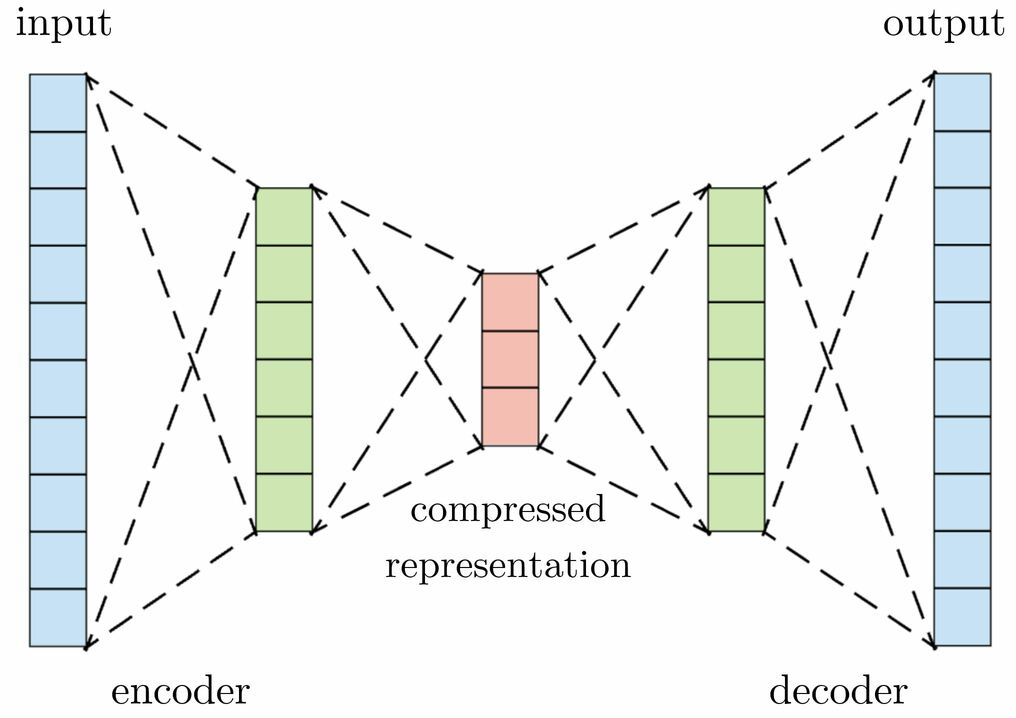
\includegraphics[scale = .19]{images/autoencodeer3.JPG}
            \vspace{-2mm}
        \end{center}
        The decoder struggles to capture anomalous patterns, and the reconstruction error acts as a score to detect anomalies.
        \\
        \smallskip
        Autoencoders can also be used for image processing, dimension reduction, and information retrieval.
        \smallskip

        \textbf{Hidden Markov Model} - uses observed events $O$ to model a set of $n$ underlying states $Q$ using $\lambda = (A,B,\pi)$
        \begin{itemize}[label={--},leftmargin=4mm]
            \itemsep -.4mm
            \item $A$ - $n\times n$ matrix of transition probabilities from state $i$ to $j$ \item $B$ - sequence of likelihoods of emitting $o_t$ in state $i$
            \item $\pi$ - initial probability distribution over states
        \end{itemize}
        HMMs can calculate $P(O|\lambda)$, find the best hidden state sequence Q, or learn the parameters $A$ and $B$.
        Anomalies are observations that are unlikely to occur across states.

        \smallskip
        HMMs can be applied to many problems such as signal processing and part of speech tagging.

        % \newpage
        % ----------------------------------------------------------------
        \textcolor{white}{.}\vspace{-5mm}\\ % Add space above column
        \section{Time Series}
        Extracts characteristics from time-sequenced data, which may exhibit the following characteristics:
        \begin{itemize}[label={--},leftmargin=4mm]
            \itemsep -.4mm
            \item Stationarity - statistical properties such as mean, variance, and auto correlation are constant over time
            \item Trend - long-term rise or fall in values
            \item Seasonality - variations associated with specific calendar times, occurring at regular intervals less than a year
            \item Cyclicality - variations without a fixed time length, occurring in periods of greater or less than one year
            \item Autocorrelation - degree of linear similarity between current and lagged values
        \end{itemize}


        CV must account for the time aspect, such as for each fold $F_x$:
        \begin{itemize}[label={--},leftmargin=4mm]
            \itemsep -.4mm
            \item Sliding Window - train $F_1$, test $F_2$, then train $F_2$, test $F_3$
            \item Forward Chain - train $F_1$, test $F_2$, then train $F_1, F_2$, test $F_3$
        \end{itemize}

        \textbf{Exponential Smoothing} - uses an exponentially decreasing weight to observations over time, and takes a moving average. The time $t$ output is $s_t = \alpha x_t + (1-\alpha)s_{t-1}$, where  $0 < \alpha < 1$.
        \smallskip

        \textbf{Double Exponential Smoothing} - applies a recursive exponential filter to capture trends within a time series
        \begin{center}
            \vspace{-2.5mm}
            $s_t = \alpha x_t + (1-\alpha)(s_{t-1} + b_{t-1})$\\
            $b_t = \beta (s_t - s_{t-1}) + (1-\beta)b_{t-1}$\\
            \vspace{-2mm}
        \end{center}
        Triple exponential smoothing adds a third variable
    $\gamma$ that accounts for seasonality.
        \smallskip

        \textbf{ARIMA} - models time series using three parameters $(p,d,q)$:
        \begin{itemize}[label={--},leftmargin=4mm]
            \itemsep -.4mm
            \item Autoregressive - the past $p$ values affect the next value

            \item Integrated - values are replaced with the difference between current and previous values, using the difference degree $d$ (0 for stationary data, and 1 for non-stationary)

            \item Moving Average - the number of lagged forecast errors and the size of the moving average window $q$
        \end{itemize}

        \textbf{SARIMA} - models seasonality through four additional seasonality-specific parameters: $P$, $D$, $Q$, and the season length $s$
        \smallskip

        \textbf{Prophet} - additive model that uses non-linear trends to account for multiple seasonalities such as yearly, weekly, and daily. Robust to missing data and handles outliers well.\\ Can be represented as: $y(t) = g(t) + s(t) + h(t) + \epsilon(t)$, with four distinct components for the growth over time, seasonality, holiday effects, and error. This specification is similar to a generalized additive model.
        \smallskip

        \textbf{Generalized Additive Model} - combine predictive methods while preserving additivity across variables, in a form such as
    $y = \beta_0 + f_1(x_1) + \cdots + f_m(x_m)$, where functions can be non-linear. GAMs also provide regularized and interpretable solutions for regression and classification problems.

        %%%%%%%%%%%%%%%%%%%%%%
        \section{Naive Bayes}
        Classifies data using the label with the highest conditional probability, given data $a$ and classes $c$. Naive because it assumes variables are independent.

        \textbf{Bayes' Theorem} $ P({c_i}|{a})  = \frac{P({a}|{c_i})P({c_i})}{P({a})}$

        \textbf{Gaussian Naive Bayes} - calculates conditional probability for continuous data by assuming a normal distribution

        % \columnbreak
        %------------------------------------------------------
        \textcolor{white}{.}\vspace{-5mm}\\ % Add space above column
        \section{Statistics}
    $\boldsymbol p$\textbf{-value} - probability that an effect could have occurred by chance. If less than the significance level $\alpha$, or if the test statistic is greater than the critical value, then reject the null.

        \textbf{Type I Error} (False Positive $\alpha$) - rejecting a true null

        \textbf{Type II  Error} (False Negative $\beta$)  - not rejecting a false null

        Decreasing Type I Error causes an increase in Type II Error

        \textbf{Confidence Level} (1 - $\alpha$) - probability of finding an effect that did not occur by chance and avoiding a Type I error

        \textbf{Power} (1 - $\beta$) - probability of picking up on an effect that is present and avoiding a Type II Error

        \textbf{Confidence Interval} - estimated interval that models the long-term frequency of capturing the true parameter value

    $\boldsymbol{z}$\textbf{-test} - tests whether normally distributed population means are different, used when $n$ is large and variances are known
        \vspace{-.5mm}
        \begin{itemize}[label={--},leftmargin=4mm]
            \itemsep -.4mm
            \item z-score - the number of standard deviations between a data point $x$ and the mean $\to \frac{x - \mu}{\sigma}$
        \end{itemize}
        \vspace{-.5mm}
    $\boldsymbol{t}$\textbf{-test} - used when population variances are unknown, and converges to the $z$-test when $n$ is large
        \vspace{-.5mm}
        \begin{itemize}[label={--},leftmargin=4mm]
            \itemsep -.4mm
            \item t-score - uses the standard error as an estimate for population variance $\to \frac{x - \mu}{s/\sqrt{n}}$
        \end{itemize}
        \vspace{-1mm}
        \textbf{Degrees of Freedom} - the number of independent (free) dimensions needed before the parameter estimate can be determined

        \textbf{Chi-Square Tests} - measure differences between categorical variables, using $\chi^2$ = $\sum \frac{observed - expected}{expected}$ to test:
        \begin{itemize}[label={--},leftmargin=4mm]
            \itemsep -.4mm
            \item Goodness of fit - if samples of one categorical variable match the population category expectations
            \item Independence -  if being in one category is independent of another, based off two categories
            \item Homogeneity - if different subgroups come from the same population, based off a single category
        \end{itemize}

        \textbf{ANOVA} - analysis of variance, used to compare 3$\plus$ samples
        \begin{itemize}[label={--},leftmargin=4mm]
            \itemsep -.4mm
            \item F-score - compares the ratio of explained and unexplained variance $\to \frac{\text{between group variance}}{\text{within group variance}}$
        \end{itemize}

        \smallskip

        \textbf{Conditional Probability} $P(A \mid B) = \frac{P(A \cap B)}{P(B)}$

        If $A$ and $B$ are independent, then $P(A \cap B) = P(A) P(B)$.\\
        Note, events that are independent of themselves must have
        probability either 1 or 0.


        \textbf{Union} $P(A \cup B) = P(A) + P(B) - P(A \cap B) $

        \textbf{Mutually Exclusive} - events cannot happen simultaneously
        \smallskip

        \textbf{Expected Value} $E[X] = \sum x_i p_i$, with properties
        \begin{itemize}[label={--},leftmargin=4mm]
            \itemsep -.4mm
            \item $E[X + Y] = E[X] + E[Y]$
            \item $E[XY] = E[X]E[Y]$ if $X$ and $Y$ are independent
        \end{itemize}

        \textbf{Variance} Var$(X) = E[X^2] - E[X]^2$, with properties
        \begin{itemize}[label={--},leftmargin=4mm]
            \itemsep -.4mm
            \item Var$(X\pm Y) =$ Var$(X) +$Var$(Y) \pm 2$Cov$(X,Y)$
            \item Var$(aX \pm b) = a^2$Var$(X)$
        \end{itemize}

        \textbf{Covariance} - measures the direction of the joint linear relationship of two variables
    $\to \frac{\sum (x_i - \bar{x}) (y_i - \bar{y})}{n-1} $

        \textbf{Correlation} - normalizes covariance to provide both strength and direction of linear relationships $\to r =  \frac{Cov(x,y)}{\sigma_x \sigma_y}$
        Independent variables are uncorrelated,  though the inverse is not necessarily true

        \newcommand*{\Perm}[2]{{}^{#1}\!P_{#2}}%
        \newcommand*{\Comb}[2]{{}^{#1}C_{#2}}%
        \smallskip

        \section{A/B Testing}
        Examines user experience through randomized tests with two variants.
        The typical steps are:
        \begin{enumerate}[leftmargin=5mm]
            \itemsep -.4mm
            \item Determine the evaluation metric and experiment goals
            \item Select a significance level $\alpha$ and power threshold 1 - $\beta$
            \item Calculate the required sample size per variation
            \item Randomly assign users into control and treatment groups
            \item Measure and analyze results using the appropriate test
        \end{enumerate}

        The required sample size depends on $\alpha$, $\beta$, and the MDE
        \textbf{Minimum Detectable Effect} - the target relative minimum increase over the baseline that should be observed from a test
        \vspace{.5mm}

        \textbf{Overall Evaluation Criterion} - quantitative measure of the test's objective, commonly used when short and long-term metrics have inverse relationships
        \vspace{.7mm}

        \textbf{Multivariate Testing} - compares 3$\plus$ variants or combinations, but requires larger sample sizes

        \textbf{Bonferroni Correction} - when conducting $n$ tests,
        run each test at the $\frac{\alpha}{n}$ significance level, which lowers the false positive rate of finding effects by chance
        \vspace{.7mm}

        \textbf{Network Effects} - changes that occur due to effect spillover from other groups. To detect group interference:
        \begin{enumerate}[leftmargin=5mm]
            \itemsep -.4mm
            \item Split the population into distinct clusters
            \item Randomly assign half the clusters to the control and treatment groups $A_1$ and $B_1$
            \item Randomize the other half at the user-level and assign to control and treatment groups
                  $A_2$ and $B_2$
            \item Intuitively, if there are network effects, then the tests will have different results
        \end{enumerate}
        To account for network effects, randomize users based on time, cluster, or location
        \smallskip

        \textbf{Sequential Testing} - allows for early experiment stopping by drawing statistical borders based on the Type I Error rate. If the effect reaches a border, the test can be stopped. Used to combat \emph{peeking} (preliminarily checking results of a test), which can inflate $p$-values and lead to incorrect conclusions.

        \textbf{Cohort Analysis} - examines specific groups of users based on behavior or time and can help identify whether novelty or primacy effects are present

        \section{Miscellaneous}
        \textbf{Shapley Values} - measures the marginal contribution of each variable in the output of a model, where the sum of all Shapley values equals the total value (prediction $-$ mean prediction)

        \textbf{SHAP} - interpretable Shapley method that utilizes both global and local importance to model variable explainability

        \textbf{Permutation} - order matters  $\to \frac{n!}{(n-k)!} = \Perm{n}{k}$

        \textbf{Combination} - order doesn't matter $\to \frac{n!}{k!(n-k)!}= \Comb{n}{k}= \binom nk$

        \textbf{Left Skew} - Mean $<$ Median $\leq$ Mode

        \textbf{Right Skew} - Mean $>$ Median $\geq$ Mode

        \textbf{Probability vs Likelihood} - given a situation $\theta$ and observed outcomes $O$, probability is calculated as $P(O|\theta)$. However, when true values for $\theta$ are unknown, $O$ is used to estimate the $\theta$ that maximizes the likelihood function. That is, $L(\theta|O) = P(O|\theta)$.
    \newpage
\end{multicols}

\end{document}